\documentclass[10pt]{elsarticle}

  \usepackage{pgfplots}
\pgfplotsset{compat=newest}
%% the following commands are needed for some matlab2tikz features
\usetikzlibrary{plotmarks}
\usetikzlibrary{arrows.meta}
\usepgfplotslibrary{patchplots}
\usepackage{grffile}
\usepackage{amsmath}
\usepackage{lineno}


%\usepackage{fullpage}
\usepackage[top=1in, bottom=1in, left=0.8in, right=1in]{geometry}
\usepackage{multicol}
\usepackage{caption}
\usepackage{subcaption}
\usepackage{hyperref}
\usepackage{xcolor}
\usepackage{graphicx,psfrag}
\usepackage[pdf]{pstricks}

\definecolor{lightblue}{rgb}{.80,.9,1}
\newcommand{\hl}[1]
    {\par\colorbox{lightblue}{\parbox{\linewidth}{#1}}}

\newcommand{\defn}{\stackrel{\textrm{\scriptsize def}}{=}}

\setlength{\columnsep}{0.1pc}

\title{Numerical Scheme for the Generalised Serre-Green-Naghdi Model}
%\author{Christopher Zoppou -- \texttt{christopher.zoppou@anu.edu.au}, Dimitrios Mitsotakis -- \texttt{dmitsot@gmail.com}, Stephen Roberts -- \texttt{stephen.roberts@anu.edu.au}, Jordan Pitt}

% TIME ON EVERY PAGE AS WELL AS THE FILE NAME
\usepackage{fancyhdr}
\usepackage{currfile}
\usepackage[us,12hr]{datetime} % `us' makes \today behave as usual in TeX/LaTeX
\fancypagestyle{plain}{
\fancyhf{}
\rfoot{\emph{\footnotesize \textcopyright  Serre Notes by  J. Pitt, C. Zoppou and S. Roberts.}
 \\ File Name: {\currfilename} \\ Date: {\ddmmyyyydate\today} at \currenttime}
\lfoot{Page \thepage}
\renewcommand{\headrulewidth}{0pt}}
\pagestyle{plain}

\definecolor{mycolor1}{rgb}{0.00000,0.44700,0.74100}%
\definecolor{mycolor2}{rgb}{0.85000,0.32500,0.09800}%
\definecolor{mycolor3}{rgb}{0.92900,0.69400,0.12500}%
\definecolor{mycolor4}{rgb}{0.49400,0.18400,0.55600}%
\definecolor{mycolor5}{rgb}{0.46600,0.67400,0.18800}% 
\definecolor{mycolor6}{rgb}{0.30100,0.74500,0.93300}%
\definecolor{mycolor7}{rgb}{0.63500,0.07800,0.18400}%

\newcommand\T{\rule{0pt}{3ex }}       % Top table strut
\newcommand\B{\rule[-4ex]{0pt}{4ex }} % Bottom table strut

\newcommand\TM{\rule{0pt}{2.8ex }}       % Top matrix strut
\newcommand\BM{\rule[-2ex]{0pt}{2ex }} % Bottom matrix strut

\newcommand{\vecn}[1]{\boldsymbol{#1}}
\DeclareRobustCommand{\solidrule}[1][0.25cm]{\rule[0.5ex]{#1}{1.5pt}}

\DeclareRobustCommand{\dashedrule}{\mbox{%
		\solidrule[2mm]\hspace{2mm}\solidrule[2mm]}}

\DeclareRobustCommand{\tikzcircle}[1]{\tikz{\filldraw[#1] (0,0) circle (0.5ex);}}	
	
	
\DeclareRobustCommand{\squaret}[1]{\tikz{\draw[#1,thick] (0,0) rectangle (0.2cm,0.2cm);}}
\DeclareRobustCommand{\circlet}[1]{\tikz{\draw[#1,thick] (0,0) circle [radius=0.1cm];}}
\DeclareRobustCommand{\trianglet}[1]{\tikz{\draw[#1,thick] (0,0) --
		(0.25cm,0) -- (0.125cm,0.25cm) -- (0,0);}}
\DeclareRobustCommand{\crosst}[1]{\tikz{\draw[#1,thick] (0cm,0cm) --
		(0.1cm,0.1cm) -- (0cm,0.2cm) -- (0.1cm,0.1cm) -- (0.2cm,0.2cm) -- (0.1cm,0.1cm)-- (0.2cm,0cm);}}
\DeclareRobustCommand{\diamondt}[1]{\tikz{\draw[#1,thick] (0,0) --(0.1cm,0.15cm) -- (0.2cm,0cm) -- (0.1cm,-0.15cm) -- (0,0)  ;}}
\DeclareRobustCommand{\squareF}[1]{\tikz{\filldraw[#1,fill opacity= 0.3] (0,0) rectangle (0.2cm,0.2cm);}}

\begin{document}

\maketitle

\vspace{-0.3in}
\noindent
\rule{\linewidth}{0.4pt}

%\tableofcontents
%
%Papers Primary focus - to extend the approach outlined in Zoppou,Hank to the gSGN equations. This achieves the following goals:
%\begin{itemize}
%	\item Extension of numerical scheme (elliptic + conservation solvers) of previous papers for SGN to gSGN
%	\item Straightforward 2nd order implementation - demonstrating the use of this method
%	\item Validation of the example implementation using analytic solutions for SWWE and SGN (dam-break and soliton) and forced solutions for more general members (only showing a select few)
%	\item Method is promising : can handle discontinuities, maintain order of accuracy. However, there are additional challenges (weak disconinuities) and limiting of derivative which will be investigated in another paper. 
%\end{itemize}


%-------------------------------------------------
\section{Abstract}
%-------------------------------------------------



%-------------------------------------------------
\section{Introduction}
%-------------------------------------------------
The generalised Serre-Green-Naghdi (gSGN) equations were recently derived by \citet{Clamond-Dutykh-2018-237}, they are a set of equations that generalise the classical Serre-Green-Naghdi (SGN) derived by \citet{Serre-F-1953-857} with the addition of two parameters $\beta_1$ and $\beta_2$. The equations describe the behaviour of water waves in shallow water where the typical water depth $h_0$ is much smaller than the wavelength $\lambda$ so that the shallowness parameter $\sigma = h_0/\lambda \ll 1$. The gSGN equations are of particular interest to the wave modelling community as their dispersion relation well approximates the dispersion relationship of the linear wave theory [], with the choice of $\beta$ values allowing for the dispersion relationship of the gSGN to be accurate up to $\mathcal{O}\left(\sigma^2\right)$ terms, $\mathcal{O}\left(\sigma^4\right)$ terms and even $\mathcal{O}\left(\sigma^6\right)$ terms. Therefore, these equations are a great way to study the behaviour of water waves as higher powers of $\sigma$ are retained in the wave model. 

In previous work we have developed and validated numerical methods for a conservative reformulation of the SGN equations \cite{Zoppou-2014,Zoppou-etal-2016,Zoppou-etal-2017,Pitt-2019}. These numerical methods have all been based on the overall scheme which solves an auxiliary elliptic equation containing only spatial derivatives, to obtain all the primitive variables in the conservation equation, and then updating the conservation equation using a finite volume method. The central benefit of the approach is the replication of the conservation of the SGN equations \cite{Pitt-2019} and the robustness of the method in the presence of steep gradients \cite{Pitt-2018-61}. The approach has been shown to produce the theoretical accuracy of the underlying methods up to third-order \cite{Zoppou-etal-2017,Pitt-2019} with the desired conservation and linear dispersion properties \cite{Pitt-2019}. The approach has also been successfully extended to include the effects of varying bathymetry and allow the presence of dry beds \cite{Pitt-2019}.  

As demonstrated by \citet{Clamond-Dutykh-2018-237}, the gSGN also possesses a conservation reformulation and thus the technique described above for the SGN equations \cite{Zoppou-2014,Zoppou-etal-2016,Zoppou-etal-2017,Pitt-2019} can be extended to the gSGN equations. The success of this technique for the SGN equations makes this an attractive option and would allow for an explicit, robust and conservative method for the gSGN equations with a straight forward implementation. Hence, the goal of this paper is the description of an extension to the numerical scheme of \citet{Zoppou-etal-2017} for the newly developed generalised Serre-Green-Naghdi (gSGN) equations \cite{Clamond-Dutykh-2018-237}. 

This paper begins by introducing the gSGN and highlighting their important properties with regards to the developed numerical scheme. The overall numerical scheme of \citet{Zoppou-etal-2017} is then described, with a straightforward second-order implementation of the method used as an example method. 

This example numerical method is then validated against analytic solutions of the SGN and the Shallow Water Wave Equations (SWWE), demonstrating its convergence rate and conservation properties. Additionally, forced solutions are used to validate that all terms in the gSGN are being accurately approximated to the correct order of accuracy. Forced solutions are necessary to validate the numerical method for the more general members of this family of equations. This demonstrates the capability of the numerical scheme to produce robust and accurate numerical methods. 




%
%These equations are a generalised family of equations that are parameterised by two free variables $\beta_1$ and $\beta_2$ and possess both the SGN equations as well as the Shallow Water Wave Equations (SWWE) as members. Additionally, they admit a family of improved dispersion Serre-Green-Naghdi (iSGN) equations \cite{Clamond-et.al-2017-245}. Together this means that the gSGN provides an opportunity for the method to be applied to improved dispersion equations whilst also allowing the method to switch between the SGN and the SWWE to simulate the onset of wave-breaking as performed by \citet{Tissier-2011} and \citet{Filippini-etal-2016-381} [] for their splitting approaches. Thus the application of the method to these equations addresses some of the key areas of interest not handled in previous papers. 
%
%Furthermore, the gSGN equations present a number of challenges beyond those of the SGN equations to the development of a numerical method. Of particular note, is the presence of the discontinuous solutions of the SWWE [] and the presence of weak discontinuities of the regularised Shallow Water Wave Equations (rSWWE) \cite{Pu-2018-1361} which are a subfamily of equations inside the gSGN. The SWWE have been solved in numerous ways [], with finite volume methods being particularly successful even in the presence of discontinuities []. This makes extensions of the finite volume based methods of \cite{Hank-etal-2010-2034,Zoppou-etal-2017} particularly desirable for these equations. Therefore, in this paper we propose a method to solve the gSGN that relies on generalising the methods for the SGN equations presented by \citet{Zoppou-etal-2017}.
%
%We begin by introducing the equations and highlighting their important properties with regards to the developed numerical method. The overall numerical scheme of \citet{Zoppou-etal-2017} is then described, with a straightforward second-order implementation of the method used as an example method. 
%
%This example numerical method is then validated against analytic solutions of the SGN and the SWWE, demonstrating its convergence rate and conservation properties. Additionally, forced solutions are used to validate that all terms in the gSGN are being accurately approximated to the correct order of accuracy. Forced solutions are necessary to validate the numerical method for the more general members of this family of equations. This demonstrates the capability of the numerical scheme to produce robust and accurate numerical methods. 


\begin{itemize}
	\item Background
	\begin{itemize}
		\item Previous papers about numerical method
		\item Numerical method has shown promise in both SWWE and SGN equations, both obtaining the desired accuracy and being robust in presenece of steep gradients.
		\item New equations are interesting for a variety of reasons: (i) contain improved disperison, (ii) allow switching of disperison on and off as done by other SGN solvers, (iii) new equations that haven't had a robust numerical method and present some new challenges - weak discontinuity.
		\item Present how SGN elliptic/hyperbolic scheme can be extended to gSGN
		\item Provide a simple/ straightforward implementation 2nd order example
		\item validate this example, to support claims
		
		Present new method, validate it using known analytic solutions for well studied members.
		\item Validate it using forced solutions
		
		\item Dispersive wave equations to model phenomena
		\item New regularisation techniques to improve dispersive properties without requiring additional higher derivative terms (Denys - improved dispersion paper)
		\item Regularisation techniques to produce regularised shock waves - (other denys paper)
		\item The equations capture this new areas whilst possessing conservation law forms
		\item Such generalised equations will allow us to gain insight into heuristic processes such as switching off dispersion/ regularisation
	\end{itemize}
\item Contributions
\begin{itemize}
	\item Numerical illustrations, but no concrete methods with validation in literature
	\item Robust numerical method
	\item Numerical study of effect of beta values, in particular for various interesting classes
\end{itemize}
\end{itemize}



%-------------------------------------------------
\section{Generalised Serre-Green-Naghdi Equations}
%-------------------------------------------------
The gSGN equations were derived by \citet{Clamond-Dutykh-2018-237} using a Lagrangian field theory approach. These equations generalise the SGN equations that describe a depth averaged approximation to the Euler equations where $h$ is the height of the free-surface of the water, $u$ is the depth averaged velocity and $g$ is the acceleration due to gravity. The gSGN equations accomplish this by introducing two free parameters $\beta_1$ and $\beta_2$, that when fixed result in a particular member of this family of equations. 

The gSGN equations describe the conservation of mass, momentum and energy ($\mathcal{E}$) for water waves like so
\begin{subequations}
\begin{align}
\begin{split}
\dfrac{\partial h}{\partial t} + \dfrac{\partial (hu)}{\partial x} = 0
\label{eq:gSGNh}
\end{split}\\
\begin{split}
\dfrac{\partial (hu)}{\partial t} + \dfrac{\partial }{\partial x} \left( hu^2 + \frac{1}{2}gh^2 + \frac{1}{3} h^2 \Gamma \right)= 0
\label{eq:gSGNuh}
\end{split}\\
\begin{split}
\dfrac{\partial\left(\mathcal{E}\right)}{\partial t} +\dfrac{\partial}{\partial x}\left[hu\left(\frac{1}{2}u^2 + \dfrac{1}{4}\beta_1h^2\dfrac{\partial u}{\partial x}\dfrac{\partial u}{\partial x} + gh\left(1 + \frac{1}{4}\beta_2\dfrac{\partial h}{\partial x}\dfrac{\partial h}{\partial x} \right)   + \frac{1}{3} h\Gamma  \right) + \frac{1}{2}\beta_2 g h^3\dfrac{\partial h}{\partial x}\dfrac{\partial u}{\partial x} \right] = 0
\label{eq:gSGNE}
\end{split}
\end{align}
where
\begin{align}
\Gamma &= \frac{3}{2}\beta_1h \left[\frac{\partial u}{\partial x}\frac{\partial u}{\partial x} - \frac{\partial^2 u}{\partial x \partial t} - u\frac{\partial^2 u}{\partial x^2}\right] - \frac{3}{2} \beta_2 g\left[h \frac{\partial^2 h}{\partial x^2} + \frac{1}{2} \frac{\partial h}{\partial x}\frac{\partial h}{\partial x} \right]\\
\mathcal{E} &=\frac{1}{2}hu^2 + \dfrac{1}{4}\beta_1 h^3 \dfrac{\partial u}{\partial x}\dfrac{\partial u}{\partial x} + \frac{1}{2}gh^2\left(1 + \frac{1}{2}\beta_2 \dfrac{\partial h}{\partial x} \dfrac{\partial h}{\partial x}\right).
\end{align}
\label{eq:gSGN}
\end{subequations}
When $\beta_1 = \beta_2 = 0$ the SWWE equations are obtained, whilst when $\beta_1 = 2/3$ and $\beta_2 = 0$ the SGN equations are recovered. 

Equations \eqref{eq:gSGN} hold for all $\beta$ values provided the solutions are sufficiently smooth. However, for particular $\beta$ values, for example those corresponding to the SWWE, it is possible to obtain non-smooth solutions for any pair of these equations that no longer satisfy all three equations simultaneously \cite{Pu-2018-1361}. Typically, since the mass and momentum equations are solved this results in dissipation of energy around discontinuities in solutions of the SWWE []. 

Since \eqref{eq:gSGN} are in conservation law form, when all solutions are sufficiently smooth and thus all equations hold simultaneously, the total amounts of all quantities remain constant in time if the system is closed. This can be seen by integrating \eqref{eq:gSGN} over the domain, and observing that the temporal derivative of the spatial integrals of mass ($h$), momentum ($uh$) and energy ($\mathcal{E}$) is zero when there is no flux across the domain boundaries. The conservation properties of numerical solutions will be used to validate the numerical method and its solutions. 

\subsection{Dispersion Relation of the Linearised gSGN}
The linear dispersion properties of water wave equations have been of particular interest \cite{Filippini-etal-2016-381,Clamond-et.al-2017-245,DoCarmo-2019-125}, as the scope of wave modelling expands to include dispersive effects. Indeed, the gSGN equations are of particular interest due to their dispersion relation well approximating the dispersion relation given by the linear theory for water waves []. 

To obtain the dispersion relationship of the linearised gSGN equations, \eqref{eq:gSGN} is first linearised by considering small waves on a mean flow depth $h_0$ and mean flow velocity $u_0$. The dispersion relationship of the linearised gSGN equations is then obtained by seeking travelling wave solutions of the form $\exp\left(i (k x - \omega t)\right)$ as was done by \citet{Zoppou-etal-2017} to obtain
\begin{equation}
\omega^\pm = u_0 k \pm k \sqrt{gh_0} \sqrt{\dfrac{\beta_2 h_0^2 k^2 + 2}{\beta_1 h_0^2 k^2 + 2} }.
\label{eq:DispRelgSGN}
\end{equation}
This dispersion relation provides the angular frequency $\omega$ of these travelling wave solutions of the linearised gSGN equations for waves with wavenumber $k$. The dispersion relation has a positive and negative branch corresponding to the direction of these waves which is denoted by the superscript on $\omega$. This dispersion relation \eqref{eq:DispRelgSGN} is equivalent to the dispersion relation derived by \citet{Clamond-Dutykh-2018-237} for the gSGN when $u_0 = 0$. 

The dispersion relation of the gSGN approximates the dispersion relationship of water, as can be seen by comparing their power series approximations [], as done below
\begin{align}
&\omega^\pm = \left(u_0 \pm \sqrt{gh_0}\right) k \pm  \frac{-1}{4}\sqrt{gh_0} k^3 h_0^2 \left(\beta_1 - \beta_2\right) \pm \dfrac{1}{32} \sqrt{gh_0} k^5 h_0^4\left(3 \beta_1^2 -  2 \beta_2 \beta_1 -\beta_2^2 \right) + \mathcal{O}\left(k^7\right) \\
&\omega^\pm_{\text{water}} = u_0 k \pm \sqrt{gk \tanh\left(k h_0\right)} = \left(u_0 \pm \sqrt{gh_0}\right) k \pm  \frac{-1}{6} h_0^2 k^3 \sqrt{gh_0} \pm \frac{19}{360} h_0^4 k^5 \sqrt{gh_0} + \mathcal{O}\left(k^7\right).
\end{align}
Which is accurate up to the $k$ term for all $\beta$ values, accurate in the $k^3$ term when $\beta_1 = \beta_2 + 2/3$ and accurate in the $k^5$ term when $\beta_1 = \beta_2 + 2/3$ and $\beta_2 = 2/15$ []. Therefore, by solving one equation we can compare the effect of including different accuracies of the dispersion relationship and their effect on physical phenomena. 



From the dispersion relation \eqref{eq:DispRelgSGN}, the phase speed $v_p$ and the group speed $v_g$ can be derived as follows
\begin{subequations}
\begin{align}
v^\pm_p &= \frac{\omega^\pm}{k} = u_0 \pm  \sqrt{gh_0} \sqrt{\dfrac{\beta_2 h_0^2 k^2 + 2}{\beta_1 h_0^2 k^2 + 2} },\\
v^\pm_g &= \frac{\partial \omega^\pm }{\partial k}= u_0  \pm  \sqrt{gh_0} \sqrt{\dfrac{\beta_2 h_0^2 k^2 + 2}{ \beta_1 h_0^2 k^2 + 2} } \left[1 +  \dfrac{\beta_2 - \beta_1 }{\left(\frac{1}{2}\beta_2 h_0^2 k^2 +1\right)\left( \left( \beta_1 - \frac{1}{3}\right) h_0^2 k^2 + 1\right)}\right].
\end{align}
\label{eq:wavespeeds}
\end{subequations}


\subsubsection{Wave Speed Bounds}
Using phase speed bounds of the SGN equations \citet{Hank-etal-2010-2034} and \citet{Zoppou-etal-2017} applied approximate Riemann solvers such as those of \citet{Kurganov-etal-2001-707} to solve the SGN. Thus, if the gSGN can also be shown to have bounded phase speeds then similar methods can be applied to solve the gSGN. 

To demonstrate that the phase speeds are bounded, observe that when $\beta_1 \ge 0$, $\beta_2 \ge 0$ and $h_0 k \ge 0$ then
\begin{equation*}
f_1(h_0k) = \dfrac{\beta_2 \left(h_0 k\right)^2 + 2}{\beta_1 \left(h_0 k\right)^2 + 2},
\end{equation*}
is a monotone function over $h_0 k$. This can be seen by reformulating and taking the derivative with respect to $h_0 k$, to obtain that 
\begin{equation*}
 \dfrac{\partial \left(f_1(h_0k)\right)}{\partial \left(h_0 k\right)} = \left[\dfrac{\beta_2}{\beta_1} - 1\right] \dfrac{4\left(h_0 k\right)}{\beta_1\left( \dfrac{4}{\beta_1} + \left(h_0 k\right)^2\right)^2}.
\end{equation*}
The derivative is greater than $0$ and thus monotone non-increasing if $\beta_2 \le \beta_1$ and less than $0$ and thus monotone non-decreasing if $\beta_2 \ge  \beta_1$  given the initial assumptions. Therefore, under the initial assumptions $v^+_p$ is monotone non-decreasing and $v^-_p$ is monotone non-increasing when $\beta_2 \le  \beta_1$ and $v^+_p$ is monotone non-increasing and $v^-_p$ is monotone non-decreasing when $\beta_2 \ge  \beta_1$. 

In addition to the monotonicity of $v^\pm_p$ when $k \rightarrow 0$ then $v^\pm_p \rightarrow u_0 \pm \sqrt{gh_0}$ whilst as $k \rightarrow \infty$ then $v^\pm_p \rightarrow u_0 \pm \sqrt{gh_0} \sqrt{{\beta_2}/ \beta_1 }$. Therefore, $v^\pm_p$ is monotonic and bounded at the limits of the domain, and thus bounded for all $\beta$ values provided that $\beta_1 = 0$ only when $\beta_2 = 0$, otherwise the $k \rightarrow \infty$ limit, is no longer bounded. Therefore, the methods of \citet{Hank-etal-2010-2034} and \citet{Zoppou-etal-2017} for the SGN equations can be extended to the gSGN as wavespeeds are bounded.

In addition to wavespeed bounds we also have the following chain of inequalities when ${\beta_2} \le \beta_1$ 
\begin{equation}
u_0 -  \sqrt{gh_0} \le  v^-_p \le u_0 - \sqrt{gh_0} \sqrt{\dfrac{\beta_2}{ \beta_1}} \le u_0 \le u_0 + \sqrt{gh_0} \sqrt{\dfrac{\beta_2}{\beta_1}} \le   v^+_p  \le u_0 +   \sqrt{gh_0}.
\label{eq:wavespeedbound1}
\end{equation}
We designate this region of $\beta$ values, as `Region 1', it is characterised by either lack of dispersion when $\beta_2 =  \beta_1$ or trailing discursive waves when $\beta_2 <  \beta_1$. Region 1 includes the SWWE, the SGN, and the iSGN family and this behaviour matches the behaviour of the dispersion given by the linear theory for water waves \cite{Whitham-1967-399}. 

When ${\beta_2} >  \beta_1 $ the inequality chain becomes
\begin{equation}
u_0 - \sqrt{gh_0} \sqrt{\dfrac{\beta_2}{ \beta_1}} \le v^-_p \le u_0 -  \sqrt{gh_0} \le  u_0 \le u_0 + \sqrt{gh_0} \le   v^+_p  \le u_0 +  \sqrt{gh_0} \sqrt{\dfrac{\beta_2}{ \beta_1}}
\label{eq:wavespeedbound2}
\end{equation}
This will be denoted as `Region 2', it is characterised by advancing dispersive waves. Advancing dispersive waves are not observed for water waves, and thus none of the equations or family of equations of interest lie in this region. Hence, the study in this paper will be restricted to Region 1.   

The regions, location of important members and families of equations in terms of $\beta$ values is summarised in Figure \ref{Fig:WaveSpeedReg}.
%
\begin{figure}
	\centering
	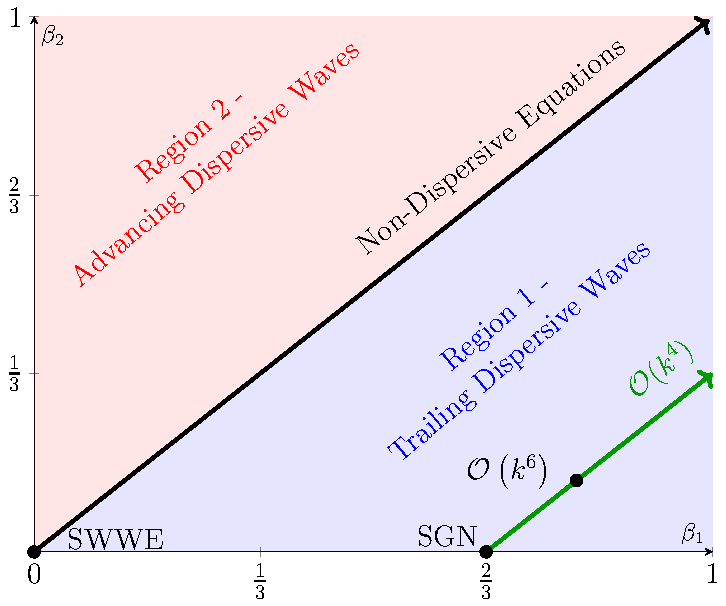
\includegraphics[width=0.4\textwidth]{./Figures/Explanation/BetaPlotAll.pdf}
	\caption{Phase speed regions of gSGN in terms of $\beta_1$ and $\beta_2$ showing important families of equations and particular members of these families.}
	\label{Fig:WaveSpeedReg}
\end{figure}


%-------------------------------------------------
\subsection{Alternative Conservative Form of the gSGN}
%-------------------------------------------------
\citet{Clamond-Dutykh-2018-237} demonstrated a rearrangement of \eqref{eq:gSGNuh} for the gSGN, in an analogous way to the reformulations of SGN \cite{Hank-etal-2010-2034,Li-2014-169,Zoppou-etal-2017}. The purpose of this reformulation is to remove the mixed spatial-temporal derivative in the flux term, which is difficult to treat numerically. This reformulation is obtained by introducing a new conserved quantity $G$
\begin{gather*}
G = hu - \frac{\beta_1}{2} \dfrac{\partial }{\partial x} \left ( h^3 \dfrac{\partial u}{\partial x} \right ).
\end{gather*}
and thus \eqref{eq:gSGNuh} can be written in conservation law form for $G$ as
\begin{gather*}\label{eq:G_momentum}
\dfrac{\partial G }{\partial t}  + \dfrac{\partial}{\partial x} \left ( uG + \dfrac{gh^2}{2} - \beta_1 h^3\dfrac{\partial u}{\partial x}\dfrac{\partial u}{\partial x}  - \frac{1}{2} \beta_2 g h^2  \left[h\frac{\partial^2 h}{\partial x^2} + \frac{1}{2}\frac{\partial h}{\partial x}\frac{\partial h}{\partial x}\right]\right ) = 0
\end{gather*}
When $\beta_1 = 2/3$ then $G$ is the same conserved quantity introduced for the SGN equations \cite{Hank-etal-2010-2034,Li-2014-169,Zoppou-etal-2017}.

This reformulation, provides the gSGN equations in conservation law form for both $h$ and the new conserved quantity $G$. Thus the conservative gSGN equations are
\begin{subequations}
\begin{gather}
\dfrac{\partial h}{\partial t} + \dfrac{\partial (uh)}{\partial x} = 0
\label{eq:gSGN_Gh}
\end{gather}
\begin{gather}
\dfrac{\partial G }{\partial t}  + \dfrac{\partial}{\partial x} \left ( uG + \dfrac{gh^2}{2} - \beta_1 h^3\dfrac{\partial u}{\partial x}\dfrac{\partial u}{\partial x}  - \frac{1}{2} \beta_2 g h^2  \left[h\frac{\partial^2 h}{\partial x^2} + \frac{1}{2}\frac{\partial h}{\partial x}\frac{\partial h}{\partial x}\right]\right ) = 0.
\label{eq:gSGN_GG}
\end{gather}
with
\begin{gather}\label{eq:G_divergent}
G = uh - \frac{\beta_1}{2}\dfrac{\partial }{\partial x} \left ( h^3 \dfrac{\partial u}{\partial x} \right ).
\end{gather}
\label{eq:gSGN_G}
\end{subequations}

Now that the gSGN equations are written in conservation law form and have a bound on the wave speeds, they can be solved numerically using the hybrid finite volume techniques described by \citet{Zoppou-etal-2017}.

\section{Numerical Scheme}
The proposed numerical scheme for the gSGN extends those previously published for the SGN equations \cite{Hank-etal-2010-2034,Zoppou-etal-2017} to allow any $\beta$ values and the associated additional terms. We will first describe a broad overview of the scheme, that serves as a general framework with which to build a variety of different numerical methods. We will then provide the simplest second-order implementation of this scheme in detail. With previous [] studies showing the sufficiency and necessity of second-order methods for the SGN equations. 


\subsection{Overview}
The heart of these hybrid finite volume methods for the gSGN equations is the finite volume method used to solve the equations in conservation law form. The finite volume method solves equations of the form 
\begin{equation}
\label{eqn:Conservf}
\frac{\partial q}{\partial t} + \frac{\partial}{\partial x}\left[f(q)\right] = 0
\end{equation}
where $q$ is a generic quantity. This is the form of the gSGN equations after the reformulation \eqref{eq:gSGN_G}. The finite volume method does this by integrating \eqref{eqn:Conservf} across cells of fixed width $\Delta x$ in space and over time steps of fixed length $\Delta t$.  The midpoint of the $j^{th}$ cell is given by $x_j = x_0 + j \Delta x$ while the cell edges of the $j^{th}$ cell are given by $x_{j-1/2} = x_0 + (j - \frac{1}{2}) \Delta x$ and $x_{j+1/2} = x_0 + (j + \frac{1}{2}) \Delta x$. Likewise the $n^{th}$ time step is given by $t^n = t^0 + n \Delta t$. 

Integrating \eqref{eqn:Conservf}  over both space and time \eqref{eqn:Conservf} one obtains
\begin{equation}
\bar{q}^{n+1}_j = \bar{q}^{n}_j  +  \dfrac{\Delta t}{\Delta x}\left[F^n_{j+1/2} - F^n_{j-1/2}\right]
\label{eqn:ConsFVM}
\end{equation}
where 
\begin{equation*}
\bar{q}^n_j = \frac{1}{\Delta x} \int_{x_j - \Delta x / 2}^{x_j - \Delta x / 2} q(x,t^n) \; dx
\end{equation*}
is the average of $q$ over the $j^{th}$ cell at time $t^n$ and   
\begin{equation*}
F^n_{j\pm 1/2} =\frac{1}{\Delta t} \int_{t^n}^{t^{n+1}} f(q(x_{j\pm 1/2},t)) dt
\end{equation*}
is the average flux of $q$ across the cell edge from time $t^n$ to $t^{n+1}$. Therefore, if $F^n_{j\pm 1/2}$ can be approximated with the appropriate order of accuracy, then we have an explicit method for updating the cell average of the conserved quantities in time. 


When describing the broad overview in addition to the point-wise values defined above it is also useful to consider collections of these values over the whole domain at a particular time. Thus, we define $\vecn{q}^n$ to be the vector of $q^n_j$ values and $\bar{\vecn{q}}^n$ to be the vector of $\bar{q}^n_j$ values for all cells in the domain at time $t^n$. 

The numerical scheme for the gSGN equations based on the finite volume method \eqref{eqn:ConsFVM} then proceeds as follows by beginning at a generic $n^{th}$ time step
\begin{enumerate}
	\item Begin with the vectors of cell averages of the conserved quantities $\bar{\vecn{h}}^n$ and $\bar{\vecn{G}}^n$.
	\item Solve \eqref{eq:G_divergent} using $\bar{\vecn{h}}^n$ and $\bar{\vecn{G}}^n$ to obtain an approximation to $\bar{{\vecn{u}}}^n$, which can be written
	\[\mathcal{A}\left(\bar{\vecn{h}}^n,\bar{\vecn{G}}^n\right) = \bar{{\vecn{u}}}^n.\]
	\item Solve \eqref{eq:gSGN_Gh} and \eqref{eq:gSGN_GG} using finite volume method \eqref{eqn:ConsFVM}  with the approximate Riemann solver of \citet{Kurganov-etal-2001-707} to obtain $\bar{h}^{n+1}_j$ and $\bar{G}^{n+1}_j$ at the next time step, obtaining
	\[\mathcal{F}\left(\bar{\vecn{h}}^n,\bar{\vecn{G}}^n,\bar{{\vecn{u}}}^n\right) = \bar{\vecn{h}}^{n+1 },\bar{\vecn{G}}^{n+1}.\]
	\item However, since $\mathcal{F}$ is only first order accurate in time steps 1-3 are repeated and then appropriate order approximations to $\bar{\vecn{h}}^{n+1 }$,$\bar{\vecn{G}}^{n+1}$ are obtained using a SSP Runge Kutta method \cite{Gottlieb-etal-2003-89}. 
\end{enumerate}

This numerical scheme produces the numerical methods of \citet{Hank-etal-2010-2034}, \citet{Zoppou-etal-2017} and \citet{Pitt-2019} when $\beta_1 = -2/3$ and $\beta_2 = 0$. Additionally, when $\beta_1 = \beta_2 = 0$ the gSGN reduce to the SWWE, and this numerical scheme reduces to a finite volume method [].  

\subsection{Example Implementation}
To demonstrate the utility of this numerical scheme we present a simple second-order implementation, and then validate it in the following section. The description of this numerical method will be broken up into the above steps for simplicity and also to highlight the interchangeability of the different parts of the scheme.

\subsubsection{Step 2 - Solution of Elliptic Equation}
To solve \eqref{eq:G_divergent} with $\bar{\vecn{h}}^n$ and $\bar{\vecn{G}}^n$ to obtain $\bar{\vecn{u}}^n$ we use the observation that the cell average and the cell nodal value are equal up to second-order accuracy and thus we can use the approximation $\bar{\vecn{q}}^n \approx {\vecn{q}}^n$ for all the quantities of interest. The second-order central finite difference approximation to \eqref{eq:G_divergent} can then be written as
\begin{equation}
{\vecn{u}}^n = \vecn{A}^{-1} {\vecn{G}}^n
\label{eq:FDGeqn}
\end{equation}
where $\vecn{A}$ is a tri-diagonal matrix with the sub-diagonal, diagonal and super-diagonal are given by
\begin{align*}
A_{j,j-1} &=  -\frac{\beta_1}{2}  \left[  \dfrac{\left(h_j^n\right)^3}{\Delta x^2} -  \dfrac{3\left(h_j^n\right)^2}{2\Delta x} \dfrac{h_{j+1}^n - h_{j-1}^n}{2\Delta x}\right] \\
A_{j,j} &= h^n_j + \beta_1\dfrac{\left(h_j^n\right)^3}{\Delta x^2} \\
A_{j,j+1} &=  -\frac{\beta_1}{2}  \left[  \dfrac{\left(h_j^n\right)^3}{\Delta x^2} +  \dfrac{3\left(h_j^n\right)^2}{2\Delta x} \dfrac{h_{j+1}^n - h_{j-1}^n}{2\Delta x}\right] . 
\end{align*}

The finite difference approximation \eqref{eq:FDGeqn} can be solved with any matrix solver, for this method we use the explicit Thomas Algorithm []. This is a good method as long as the diagonals are strictly greater than zero which is the case as long as $h_{j}^n > 0$, which is the true for all the problems of interest in this paper. 

Thus as desired we have 
\begin{equation}
\mathcal{A}\left(\bar{\vecn{h}}^n,\bar{\vecn{G}}^n\right) = \vecn{A}^{-1} {\vecn{G}}^n = \vecn{u}^n = \bar{{\vecn{u}}}^n. 
\label{eq:A_secondord}
\end{equation}


\subsubsection{Reconstruction of quantities at cell boundaries}
The finite volume method of \citet{Kurganov-etal-2001-707} relies on approximations of all the terms in the spatial derivative at the cell edges $x_{j\pm1/2}$. Thus the following quantities require second-order approximations at the cell edges: $u$, $h$, $G$, $\partial u / \partial x$, $\partial h / \partial x$, $\partial^2 h / \partial x^2$. In this paper we are interested in reproducing solutions to either smooth analytic and forced solutions or the discontinuous dam-break solutions of the SWWE where only $h$, $u$ and $G$ need to be approximated. For this reason our approximations to to  $u$, $h$, $G$, will allow for discontinuities and thus use limiting while the approximations to the derivatives $\partial u / \partial x$, $\partial h / \partial x$, $\partial^2 h / \partial x^2$ will assume that these quantities are smooth and thus not require limiting.

For $h$, $u$ and $G$ to get a second-order approximation that ensures stability in the presence of discontinuities we employ slope limiting, as done previously for the SGN equations \cite{Zoppou-etal-2017}. The reconstructions for all these quantities can be summarised for a general quantity $q$ like so
\begin{align}
q^+_{j-1/2} = \bar{q}_j - \frac{\Delta x}{2} s_j & & \text{and} & &
q^-_{j-1/2} = \bar{q}_j + \frac{\Delta x}{2} s_j
\end{align}
where
\begin{equation}
s_j = \text{minmod}\left(\theta \dfrac{\bar{q}_j - \bar{q}_{j-1}}{\Delta x},  \dfrac{\bar{q}_{j+1} - \bar{q}_{j-1}}{2\Delta x},\theta \dfrac{\bar{q}_{j+1} - \bar{q}_{j}}{\Delta x}\right).
\end{equation}
The minmod function is defined as follows
\begin{equation}
\text{minmod}\left(a,b,c\right) = \left\lbrace \begin{array}{l c l}
\min{\left(a,b,c\right)} & \text{when} & a<0, b<0, c<0 \\
\max{\left(a,b,c\right)} & \text{when} & a>0, b>0, c>0 \\
0 & & \text{otherwise}
\end{array} \right. . 
\end{equation}
This gives a reconstruction at the cell level for each cell edge, so cell $j$ gives rise to $q^+_{j-1/2}$ and $q^-_{j+1/2} $ while cell $j+1$ gives rise to $q^+_{j+1/2}$ and $q^-_{j+3/2}$ all of which are required by the flux approximation.

For $\partial u / \partial x$, $\partial h / \partial x$ and $\partial^2 h / \partial x^2$ we assume that the quantities are smooth, and so using the appropriate order finite difference approximation at the cell edges is sufficient. We demonstrate this for cell $x_{j+1/2}$ and a general quantity $q$.

\begin{align*}
\left[\dfrac{\partial q}{\partial x} \right]_{j+1/2} &= \dfrac{q_{j+1} - q_j}{\Delta x}, \\
\left[\dfrac{\partial^2 q}{\partial x^2} \right]_{j+1/2} &=  \dfrac{q_{j+2} - q_{j+1} - q_j + q_{j-1}}{2 \Delta x^2} .
\end{align*}


\subsubsection{Step 3 - Finite Volume Method}
To solve \eqref{eq:gSGN_Gh} and \eqref{eq:gSGN_GG} which are both in conservation law form \eqref{eqn:Conservf} we use \eqref{eqn:ConsFVM}. Since we begin with $\bar{\vecn{h}}^n$ and $\bar{\vecn{G}}^n$, we only require an approximation to $F^n_{j\pm1/2}$ to make use of \eqref{eqn:ConsFVM} to obtain $\bar{\vecn{h}}^{n+1}$ and $\bar{\vecn{G}}^{n+1}$.

In this numerical scheme the flux approximation method described by  \citet{Kurganov-etal-2001-707} for $F^n_{j\pm1/2}$ is used. This central benefit of this scheme is that it only requires bounds on the wave speeds [].Only the calculation of the flux term $F^n_{j+1/2}$ is demonstrated as the process to calculate the flux term $F^n_{j-1/2}$ is identical but with different cells. For a general quantity $q$ the flux approximation method \cite{Kurganov-etal-2001-707} is
\begin{equation}\label{eqn:HLL_flux}
F^n_{j+\frac{1}{2}} = \dfrac{a^+_{j+\frac{1}{2}} f\left(q^-_{j+\frac{1}{2}}\right) - a^-_{j+\frac{1}{2}} f\left(q^+_{j+\frac{1}{2}}\right)}{a^+_{j+\frac{1}{2}} - a^-_{j+\frac{1}{2}}}  + \dfrac{a^+_{j+\frac{1}{2}} \, a^-_{j+\frac{1}{2}}}{a^+_{j+\frac{1}{2}} - a^-_{j+\frac{1}{2}}} \left [ q^+_{j+\frac{1}{2}} - q^-_{j+\frac{1}{2}} \right ]
\end{equation}

where $a^+_{j+\frac{1}{2}}$ and $a^-_{j+\frac{1}{2}}$ are given by the wave speed bounds and all quantities on the right hand side are computed at time $t^n$. Applying the wave speed bounds \eqref{eq:wavespeedbound1} and \eqref{eq:wavespeedbound2} we obtain
\begin{align}
a^-_{j+\frac{1}{2}} &= \min\left\lbrace 0\;,\;  u^-_{j + 1/2} - \max{\left(1 , \sqrt{\frac{\beta_2}{\beta_1}}\right)} \sqrt{g h^-_{j + 1/2}}  \;,\;u^+_{j + 1/2} -\max{\left(1 , \sqrt{\frac{\beta_2}{\beta_1}}\right)} \sqrt{g h^+_{j + 1/2}} \right\rbrace  ,\\
a^+_{j+\frac{1}{2}} &= \max\left\lbrace 0 \;,\;  u^-_{j + 1/2} + \max{\left(1 , \sqrt{\frac{\beta_2}{\beta_1}}\right)}\sqrt{g h^-_{j + 1/2}}  \;,\;u^+_{j + 1/2} + \max{\left(1 , \sqrt{\frac{\beta_2}{\beta_1}}\right)}\sqrt{g h^+_{j + 1/2}} \right\rbrace
\label{eqn:WaveSpeedBoundsFluxApprox}
\end{align}
where the $\max{\left(1 , \sqrt{\frac{\beta_2}{\beta_1}}\right)}$ accounts for the different wavespeed bounds  \eqref{eq:wavespeedbound1} and \eqref{eq:wavespeedbound2} which depend on the choice of $\beta$ values. 

The flux functions $f(q^-_{j+\frac{1}{2}})$ and $f(q^+_{j+\frac{1}{2}})$ are evaluated using the reconstructed values of the $j^{th}$ and $(j+1)^{th}$ cell respectively. From the continuity equation \eqref{eq:gSGN_Gh} we have
\begin{align*}
f\left(h^\pm_{j+\frac{1}{2}}\right) &= u^\pm_{j + 1/2}  h^\pm_{j + 1/2}.
\end{align*}

For the evolution of $G$ equation \eqref{eq:gSGN_GG} we have 
\begin{multline}
f\left(G^\pm_{j+\frac{1}{2}}\right) =  u^\pm_{j + 1/2} G^\pm_{j + 1/2}  + \frac{g}{2}\left(h^\pm_{j + 1/2} \right)^2 - \beta_1\left(h^\pm_{j + 1/2}\right)^3 \left(\left[\frac{\partial {u}}{\partial x} \right]_{j + 1/2} \right)^2 \\ - \frac{1}{2} \beta_2 g \left(h^\pm_{j + 1/2}\right)^2  \left[h^\pm_{j + 1/2}\left[\dfrac{\partial^2 h}{\partial x^2} \right]_{j+1/2} + \frac{1}{2}\left(\left[\dfrac{\partial h}{\partial x} \right]_{j+1/2}\right)^2\right].
\end{multline}
where derivatives are assumed to be smooth over the cell edge, and thus don't require different superscripts.

Since the reconstructions were given above for all these quantities, we can approximate $F^n_{j\pm1/2}$ using \eqref{eqn:HLL_flux} and thus employ \eqref{eqn:ConsFVM} to obtain $\bar{\vecn{h}}^{n+1}$ and $\bar{\vecn{G}}^{n+1}$ resulting in
\begin{equation}
\mathcal{F}\left(\bar{\vecn{h}}^n,\bar{\vecn{G}}^n,\bar{{\vecn{u}}}^n\right) =   \bar{q}^{n}_j  +  \dfrac{\Delta t}{\Delta x}\left[F^n_{j+1/2} - F^n_{j-1/2}\right] = \bar{\vecn{h}}^{n+1 },\bar{\vecn{G}}^{n+1}
\label{eq:F_secondord}
\end{equation}
as desired. 



\subsubsection{Step 4 - Runge-Kutta Time Stepping}
Combining both Steps 2 and Steps 3, provides a spatially second-order scheme with first-order time stepping. To arrive at a fully second-order method, we make use of repeating Steps 2 and Steps 3 and applying the second-order SSP Runge Kutta method \cite{Gottlieb-etal-2003-89}. Doing this we obtain the following scheme making use of the above implementation of $\mathcal{A}$ \eqref{eq:A_secondord} and $\mathcal{F}$ \eqref{eq:F_secondord}
\begin{align}
\bar{\vecn{h}}^{'},\bar{\vecn{G}}^{'} &= \mathcal{F}\left(\bar{\vecn{h}}^n,\bar{\vecn{G}}^n,\mathcal{A}\left(\bar{\vecn{h}}^n,\bar{\vecn{G}}^n\right) \right) \\
\bar{\vecn{h}}^{''},\bar{\vecn{G}}^{''} &= \mathcal{F}\left(\bar{\vecn{h}}^{'},\bar{\vecn{G}}^{'},\mathcal{A}\left(\bar{\vecn{h}}^{'},\bar{\vecn{G}}^{'}\right) \right)\\
\bar{\vecn{h}}^{n+1},\bar{\vecn{G}}^{n+1} &= \frac{1}{2}\left(\bar{\vecn{h}}^n + \bar{\vecn{h}}^{''} \right) ,  \frac{1}{2}\left(\bar{\vecn{G}}^n + \bar{\vecn{G}}^{''} \right). 
\end{align}
Hence we obtain a stable fully second-order method. 

\subsection{Courant-Frederichs-Lewy Condition}
To ensure the stability of the finite volume method \eqref{eqn:ConsFVM} the Courant-Friedrichs-Lewy (CFL) condition \cite{Courant-etal-1967-215} is used. The CFL condition is necessary for stability and ensures that time steps are small enough so that information is only transferred between neighbouring cells. For the Serre equations the CFL condition is 
\begin{equation}
\Delta t \le \frac{Cr }{\max_{j} \left\lbrace a^\pm_{j+1/2} \right\rbrace} \Delta x
\label{eqn:CFLcond}
\end{equation}
where $a^\pm_{j+1/2} $ are the wave-speed bounds used in the flux approximation \eqref{eqn:WaveSpeedBoundsFluxApprox} and $0\le Cr \le 1$ is the Courant number. 

\section{Validation}
The numerical method described above is validated using analytic solutions for particular $\beta$ values that correspond to the SGN equations and the SWWE and a forced solution. Together these tests demonstrate the ability of the method to reproduce analytic solutions to important members of the gSGN family, as well as solve the gSGN for any pair of $\beta$ values that admit wave speed bounds.

The accuracy of the numerical method will be measured using the distance between the numerical solution and the equivalent analytic or forced solution using the $L_2$ norm. While the conservation properties of the numerical method will be measured by numerically approximating the energy in the initial conditions and the numerical solution and comparing them using a measure called $C_1$.

For a quantity $q$ with a vector of its analytic or forced solution at the cell midpoints $\vecn{q}$ and the numerical solution at the cell midpoints $\vecn{q}^*$, the discrete $L_2$ norm is
\begin{equation}
\label{eqn:Conv_Error}
L_2\left(\vecn{q},\vecn{q}^*\right) = \sqrt{ \dfrac{\sum_{j = 0}  \left[q_j^2 - \left(q^*_j\right)^2 \right]}{\sum_{j = 0}  \left[q_j^2 \right]}}
\end{equation}
where the time-step superscripts were suppressed for simplicity.

For a quantity $q$ with a vector of its values at the $n^{th}$ time step $\vecn{q}^n$, the total amount of the quantity is approximated by $C(\vecn{q}^n)$. The method for this is the same as the method described by \citet{Zoppou-etal-2017}, which has a higher order of accuracy than the numerical method it is measuring. Using the numerical approximation to the total amounts, the conservation error is obtained in the following way
\begin{equation}
\label{eqn:Cons_Error}
C_1\left(\vecn{q}^0,\vecn{q}^n\right) = \left \lbrace \begin{array}{l c r}
\dfrac{\left | C(\vecn{q}^0) - C(\vecn{q}^n) \right |}{\left| C(\vecn{q}^0) \right|}&,& \left| C(\vecn{q}^0) \right| > 0 \T \\
\left | C(\vecn{q}^0) - C(\vecn{q}^n) \right |&,& \left| C(\vecn{q}^0) \right| = 0 
\end{array} \right. .
\end{equation}

\begin{itemize}
	\item Analytic solutions - we recover them (conservation and norm)
	\item Forced solutions - our numerical method can handle any combination of beta values, all terms are approximated with correct order of accuracy. Limiters on gradients off. 
\end{itemize}

\subsection{Analytic Solutions}
The analytic solutions used to validate the numerical method, are the soliton solution of the SGN equations and the dam-break solution of the SWWE. The soliton solution is a smooth travelling wave solution, that assesses the balance of the non-linear and dispersive terms in the gSGN equations. Whereas the dam-break solution of the SWWE demonstrates the robustness of the method in the presence of steep gradients. The soliton solution used in this paper, is the same as the soliton solution used for validation by \citet{Pitt-2019}, allowing for a comparison of this gSGN solver to the more specialised SGN solvers described in that paper. 

\subsubsection{Serre Equations ($\beta_1 = -2/3$ and $\beta_2 = 0$) - Solitary Travelling Wave Solution}
When $\beta_1 = -2/3$ and $\beta_2 = 0$ the gSGN are equivalent to the SGN equations which admit the following travelling wave solution
\begin{subequations}
	\begin{equation}
	h(x,t) = a_0 + a_1 \text{sech}^2\left( \kappa (x - ct) \right),
	\end{equation}
	\begin{equation}
	u(x,t) = c \left( 1- \dfrac{a_0}{h(x,t)} \right),
	\end{equation}
	where
	\begin{equation}
	\kappa = \dfrac{\sqrt{3a_1}}{2a_0 \sqrt{a_0 + a_1}}
	\end{equation}
	and
	\begin{equation}
	c = \sqrt{g\left(a_0 + a_1\right)}.
	\end{equation}
\end{subequations}

This travelling wave solution is maintained due to a balance between the dispersive terms and the non-linear terms in the momentum equation \eqref{eq:G_momentum}. Validating the numerical solutions for the gSGN solver using this solution tests the balance between these terms in \eqref{eq:G_momentum}, and allows us to verify the method's conservation of energy as the solution is smooth. To enable a comparison between the numerical method and the SGN solver of \cite{Zoppou-etal-2017} the chosen soliton parameters were $a_0 = 1$ and $a_1 = 0.7$ and the acceleration due to gravity at the earth surface, $g = 9.81 m^2/s$ was used.

The numerical solution was solved over the domain $\left[-200,200\right]$ from $t=0s$ until $t=30s$. To ensure that the SGN solution is recovered, $\beta_1 = -2/3$ and $\beta_2 = 0$. The spatial resolution was varied like so $\Delta x = 400 / (100 \times 2^{l})$, where $l$ was increased. To satisfy the Courant-Friedrichs-Lewy (CFL) condition \cite{Lax-Richtmyer-1956-267} the time step width $\Delta t = \Delta x  / \left( 2 \sqrt{g \left(a_0 + a_1\right)}\right)$ \cite{Pitt-2019} was chosen. The limiting parameter $\theta$ was set to $\theta = 1.2$, matching the numerical experiments performed by \citet{Pitt-2019}.

Example numerical solutions for $h$, $u$ and $G$ with $\Delta x = 400 / (100 \times 2^{6}) \simeq 0.06m$ are plotted in Figure \ref{Fig:Sol_Ex}. These examples demonstrate that the numerical solutions well reproduced the analytic solutions.
%
\begin{figure}
	\centering
	\begin{subfigure}{0.32\textwidth}
		\centering
		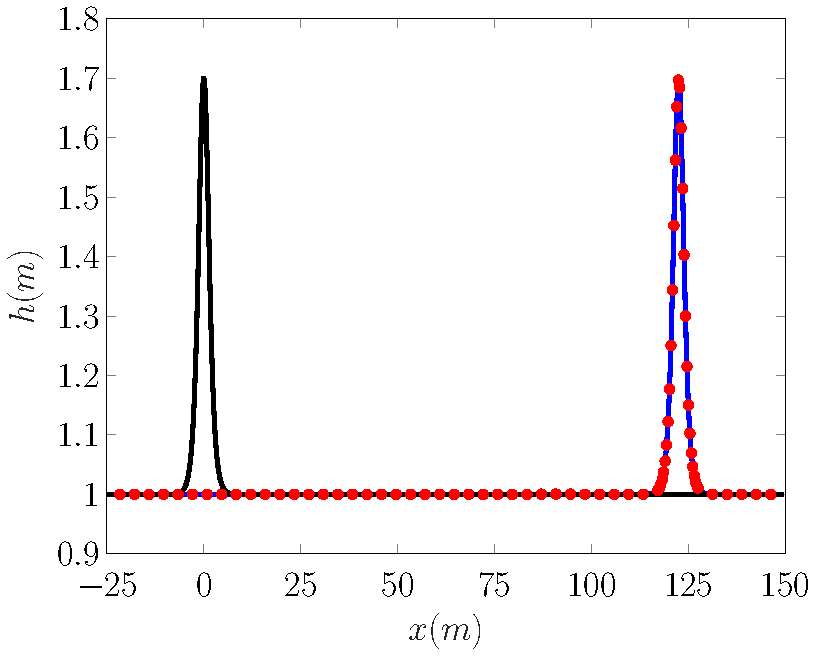
\includegraphics[width=\textwidth]{./Figures/Simulations/Validation/Serre/hEx.pdf}
		\caption{$h$}
	\end{subfigure}
	\begin{subfigure}{0.32\textwidth}
		\centering
		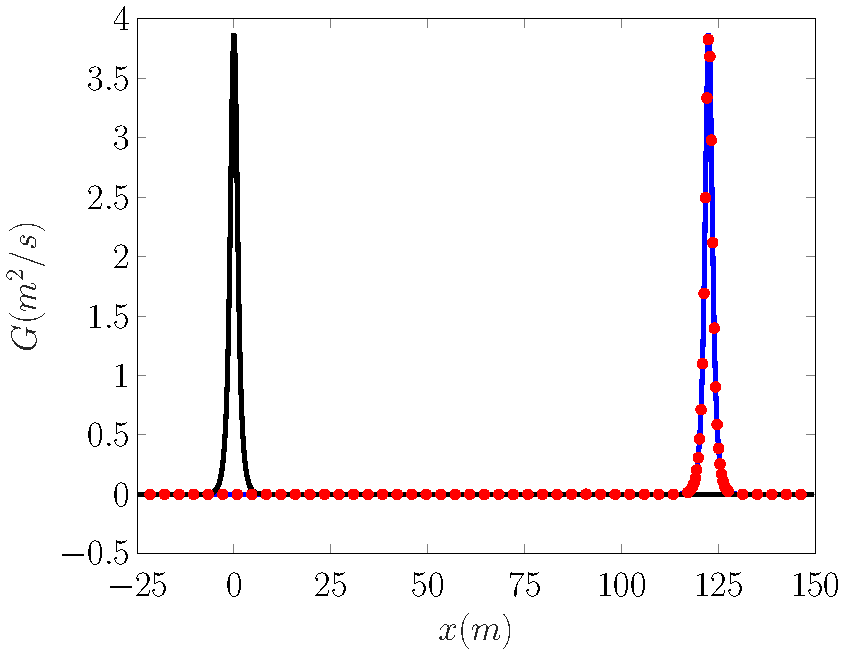
\includegraphics[width=\textwidth]{./Figures/Simulations/Validation/Serre/GEx.pdf}
		\caption{$G$}
	\end{subfigure}
	\begin{subfigure}{0.32\textwidth}
		\centering
		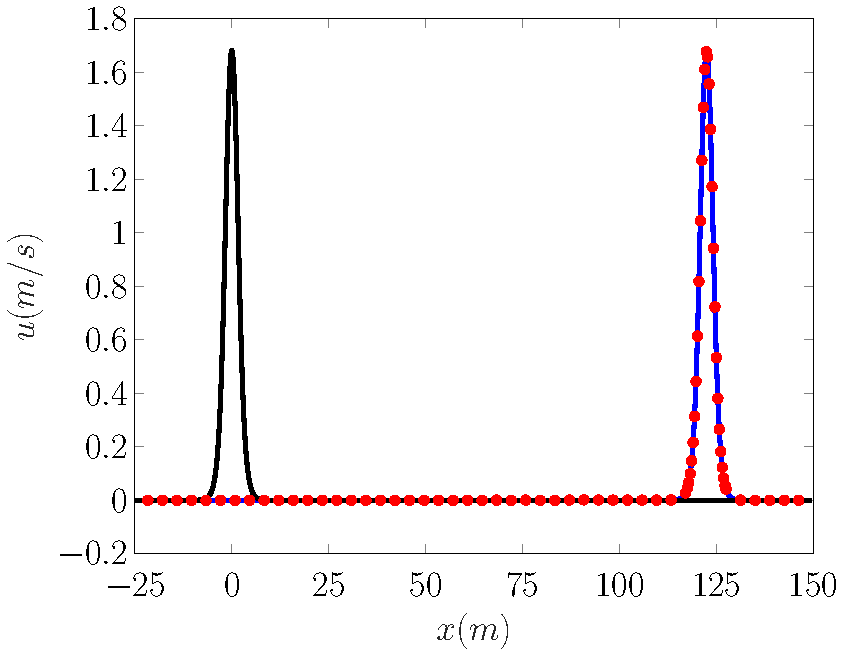
\includegraphics[width=\textwidth]{./Figures/Simulations/Validation/Serre/uEx.pdf}
		\caption{$u$}
	\end{subfigure}
	\caption{Plot of comparing initial (\solidrule), analytic solution ({\color{blue}\solidrule}), and numerical solution with $\Delta x \approx 0.06m$ (\tikzcircle{red}) at $t = 30s$.}
	\label{Fig:Sol_Ex}
\end{figure}

A comparison of many numerical solutions with varying $\Delta x$ are given in Figure \ref{Fig:Sol_Comp} for both the convergence and conservation measures. These plots demonstrate that the scheme obtains second-order convergence for all quantities of interest, after $\Delta x$ becomes small enough to properly represent the initial conditions. 

\begin{figure}
	\centering
	\begin{subfigure}{0.49\textwidth}
		\centering
		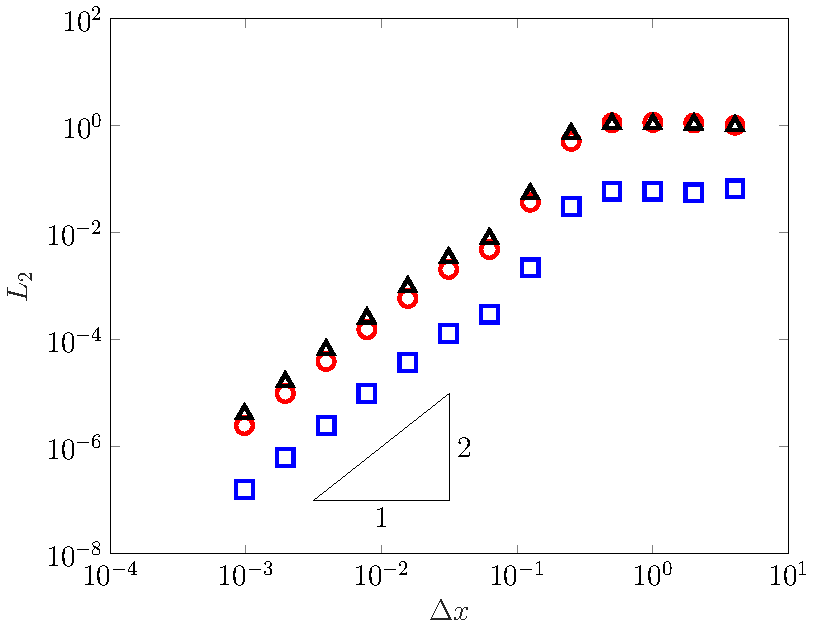
\includegraphics[width=\textwidth]{./Figures/Simulations/Validation/Serre/NormResults.pdf}
		\caption{$L_2$}
		\label{Fig:Sol_Comp_Conv}
	\end{subfigure}
	\begin{subfigure}{0.49\textwidth}
		\centering
		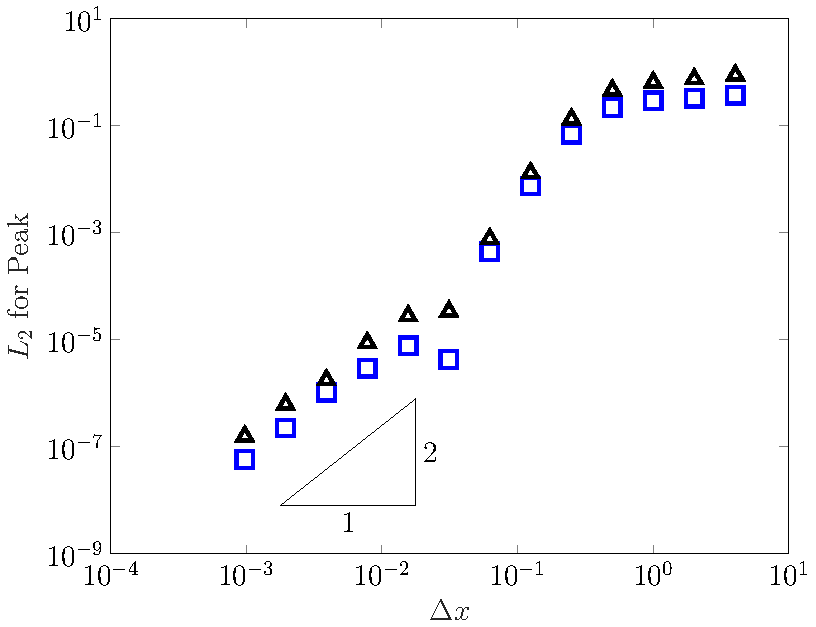
\includegraphics[width=\textwidth]{./Figures/Simulations/Validation/Serre/PeakError.pdf}
		\caption{Convergence around Peak}
		\label{Fig:Sol_Comp_Peak}
	\end{subfigure}
	\caption{Convergence plots for $h$ (\squaret{blue}) , $G$ (\circlet{red}) and $u$ (\trianglet{black}) as $\Delta x$ varies.}
	\label{Fig:Sol_Comp}
\end{figure}


\begin{figure}
	\centering
	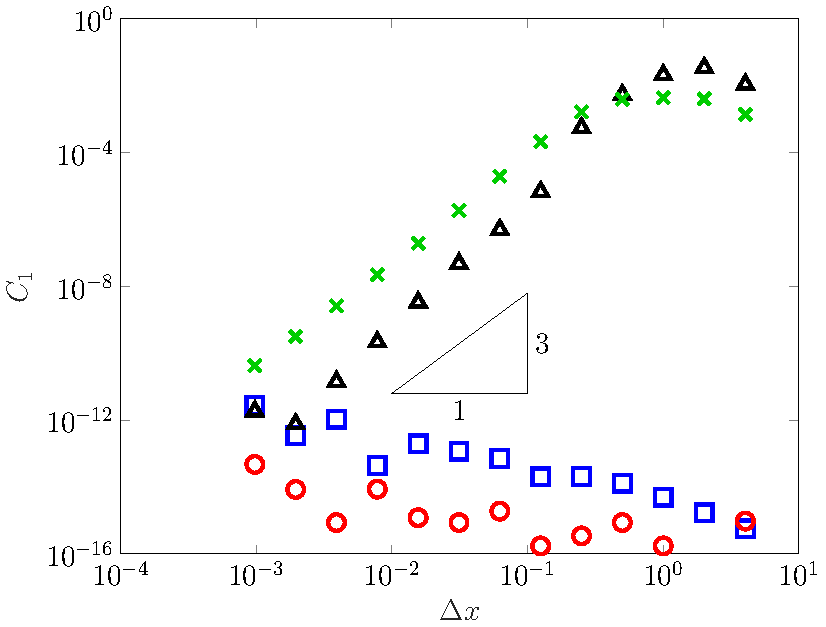
\includegraphics[width=0.49\textwidth]{./Figures/Simulations/Validation/Serre/EnergyResults.pdf}
	\caption{Conservation plot for $h$ (\squaret{blue}) , $G$ (\circlet{red}), $uh$ (\trianglet{black}) and $\mathcal{E}$ (\crosst{green!80!black}) as $\Delta x$ varies.}
	\label{Fig:Sol_Comp_Cons}
\end{figure}


\begin{figure}
	\centering
	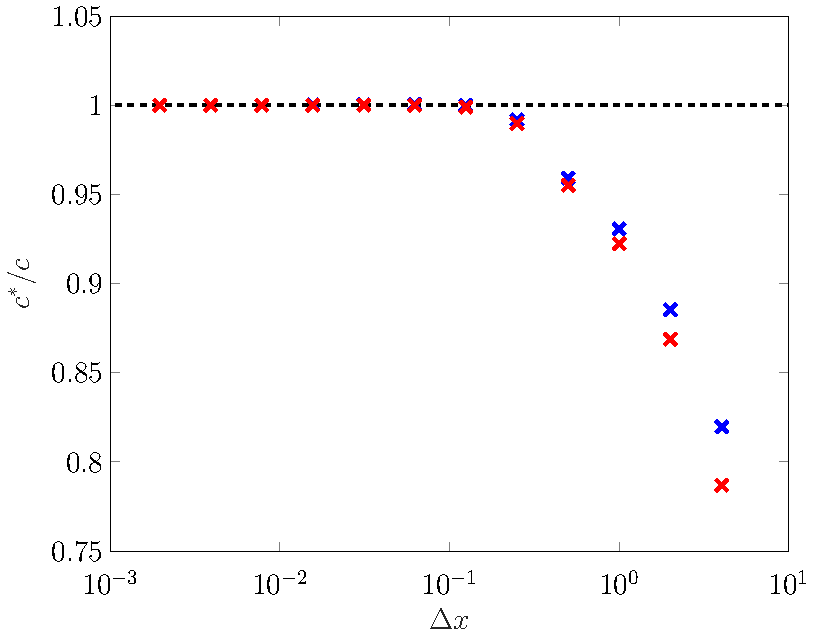
\includegraphics[width=0.49\textwidth]{./Figures/Simulations/Validation/Serre/PeakSpeedEstimates.pdf}
	\caption{Peak Speed.}
	\label{Fig:Sol_Comp_Speed}
\end{figure}

%
The conservation plot in Figure \ref{Fig:Sol_Comp_Conv} demonstrates that due to the use of the finite volume method $h$ and $G$ are conserved up to round-off error, which increases as $\Delta x$ increases. The conservation of $uh$ and $\mathcal{H}$ whilst not being at round-off error does reduce at a rate better than second-order and so the scheme possesses good convergence and conservation properties. These results agree well with the numerical solutions of \citet{Pitt-2019}, who compared various numerical methods. 

\subsubsection{SWWE ( $\beta_1= \beta_2 =0$ ) - Dam-break Solution }
When $\beta_1=\beta_2 =0$ the gSGN equations reduce to the SWWE which have an analytic solution to the dam-break problem given by the initial conditions
\begin{align}
h(x,0) & = \left\lbrace \begin{array}{c c}
h_0 & x < 0\\
h_1 & x \ge 0
\end{array} \right.  \\
u(x,0) &= 0 \\
G(x,0) &= 0.
\end{align}

The solution to the dam-break problem is given by
\begin{align}
h(x,t) &= \left \lbrace \begin{array}{l c r}
h_0 &,& x \le -t\sqrt{g h_0} \\
\frac{4}{9g} \left(\sqrt{gh_0} - \frac{x}{2t}\right)^2 &,&  -t\sqrt{g h_0} < x \le t \left(u_2 - \sqrt{g h_2}\right)  \\
h_2 &,&  t \left(u_2 - \sqrt{g h_2}\right) < x \le t S_2  \\
h_1 &,&   t S_2 \le x \\
\end{array} \right.  \\
u(x,t) &= \left \lbrace \begin{array}{l c r}
0 &,& x \le -t\sqrt{g h_0} \\
\frac{2}{3} \left(\sqrt{gh_0} + \frac{x}{t}\right) &,&  -t\sqrt{g h_0} < x \le t \left(u_2 - \sqrt{g h_2}\right)  \\
u_2 &,&  t \left(u_2 - \sqrt{g h_2}\right) < x \le t S_2  \\
0 &,&   t S_2 \le x \\
\end{array} \right. .
\end{align}
%
The constant state values $h_2$ and $u_2$ and the shock speed $S_2$ can be calculated for any initial conditions by solving
\begin{align}
\label{eq:SWWEMiddleState}
h_2 &= \dfrac{h_0}{2} \left(  \sqrt{1 + 8 \left( \dfrac{2 h_2}{h_2 - h_0} \left(\dfrac{\sqrt{gh_1} - \sqrt{gh_2}}{\sqrt{gh_0}}\right)\right)^2 } - 1 \right) \\
u_2 &= 2\left(\sqrt{gh_1} - \sqrt{gh_2} \right),\\
S_2 &= \dfrac{2 h_2}{h_2 - h_1}\left(\sqrt{gh_0} - \sqrt{gh_2} \right).
\end{align}

The initial conditions as well as the analytic solution are discontinuous. Due to the discontinuities the solutions to the initial conditions are not unique, as solving any pair of the 3 conservation equations \eqref{eq:gSGN}, gives solutions with similar structures but different constant values. The solution presented above is solution of the mass and momentum equations, as these equations are the basis of the numerical method.

A number of numerical experiments were run for the dam-break problem with $h_0 = 2m$ and $h_1 = 1m$. The domain of the solution was $\left[-250,250\right]$ with a final time of $t=35s$.  The spatial resolution was varied like so $\Delta x = 500 / (1000 \times 2^{l})$, while to satisfy the CFL condition \cite{Lax-Richtmyer-1956-267} the time step width $\Delta t = \Delta x  / \left( 2 \sqrt{g h_0}\right)$ was used. The limiting parameter $\theta$ was set to be $\theta = 1.0$ and the acceleration due to gravity $g = 9.81 m^2/s$ was used. 

Example numerical solutions and analytic solutions for $h$, $G$ and $u$ at the final time with the spatial resolution $\Delta x = 500 / (1000 \times 2^{4})$ are plotted in Figure \ref{Fig:DB_Ex}. These figures demonstrate that the method is robust in the presence of steep gradients and appropriately reproduces the broad structure of the analytic solution. 
%
\begin{figure}
	\centering
	\begin{subfigure}{0.32\textwidth}
		\centering
		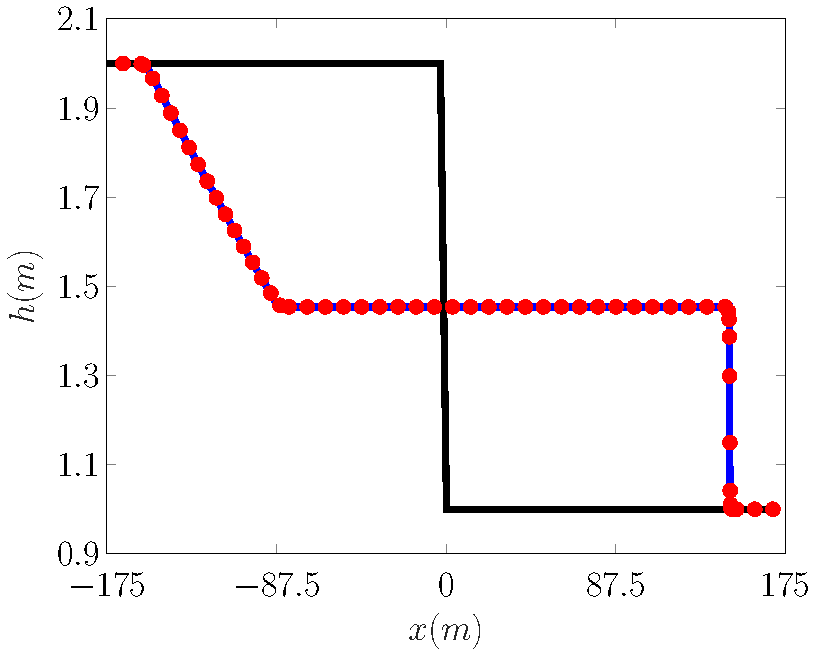
\includegraphics[width=\textwidth]{./Figures/Simulations/Validation/DBSWWE/hEx.pdf}
		\caption{$h$}
	\end{subfigure}
	\begin{subfigure}{0.32\textwidth}
		\centering
		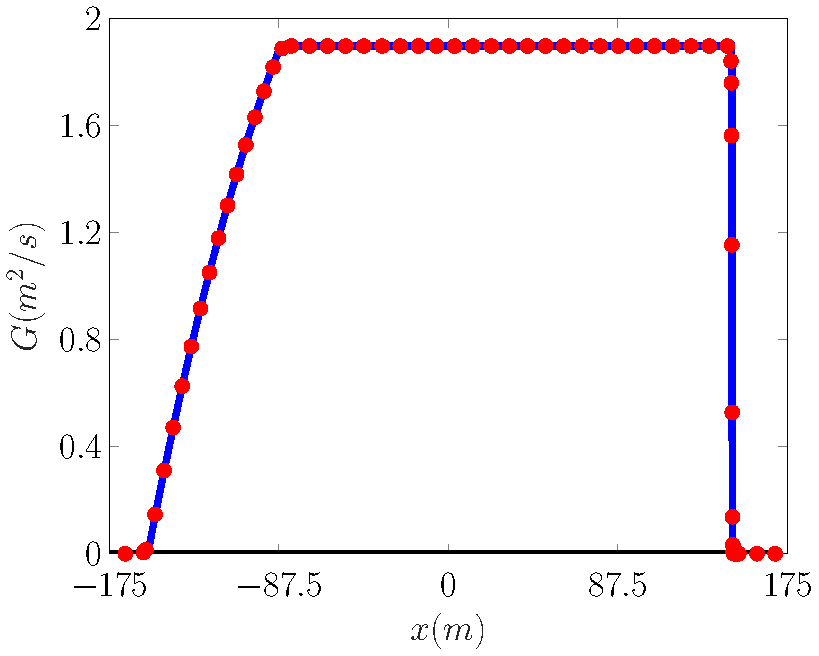
\includegraphics[width=\textwidth]{./Figures/Simulations/Validation/DBSWWE/GEx.pdf}
		\caption{$G = uh$}
	\end{subfigure}
	\begin{subfigure}{0.32\textwidth}
		\centering
		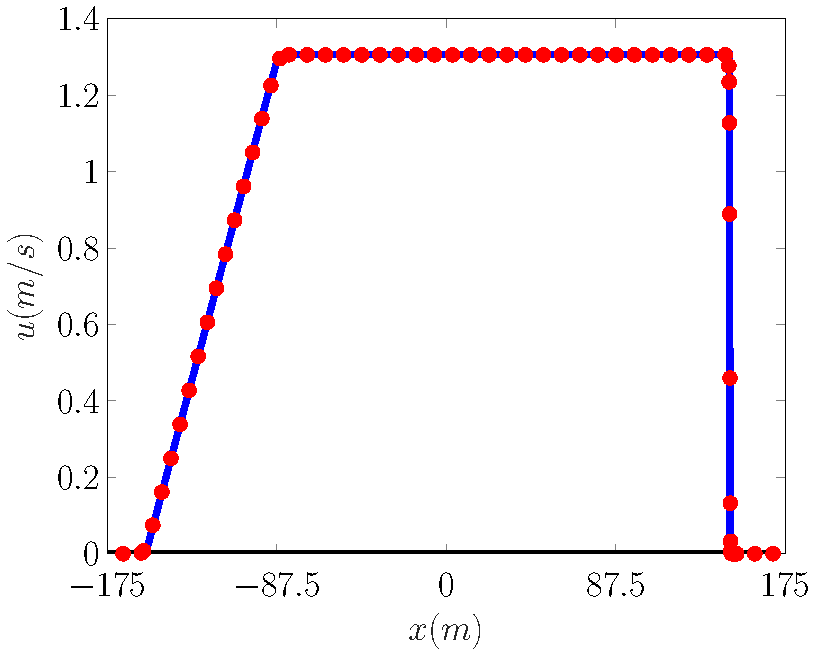
\includegraphics[width=\textwidth]{./Figures/Simulations/Validation/DBSWWE/uEx.pdf}
		\caption{$u$}
	\end{subfigure}
	\caption{Comparison of initial (\solidrule), analytic solution ({\color{blue}\solidrule}), and numerical solution with $\Delta x \approx 0.16m$ (\tikzcircle{red}) at  $t=35s$.}
	\label{Fig:DB_Ex}
\end{figure}

The central difficulty of reproducing the analytic solutions for the dam-break problem, is observed around only a few critical locations; the top of the rarefaction fan, the bottom of the rarefaction fan and the shock front. Figure \ref{Fig:Conv_Ex} demonstrates the convergence of the solutions for $h$ as $\Delta x$ changes for the top of the rarefaction fan and the shock front. 

\begin{figure}
	\centering
	\begin{subfigure}{0.45\textwidth}
		\centering
		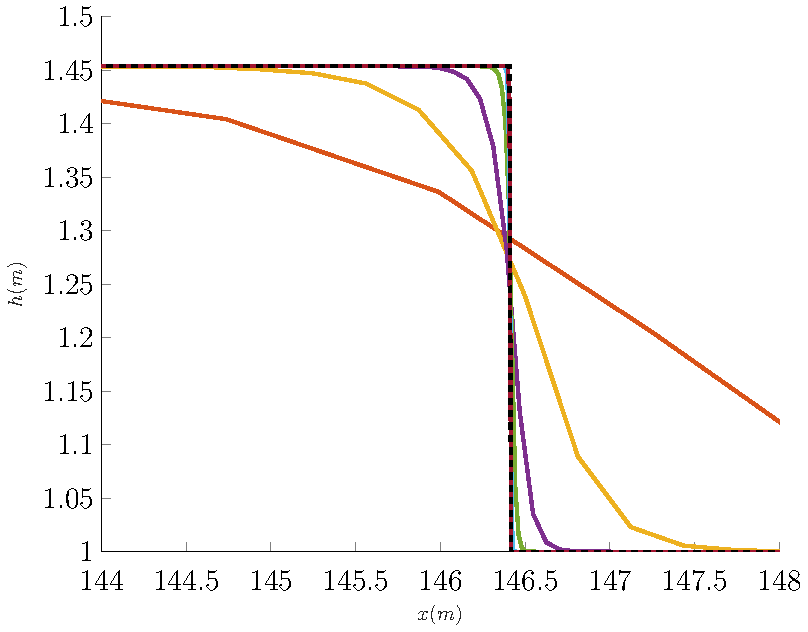
\includegraphics[width=\textwidth]{./Figures/Simulations/Validation/DBSWWE/hFront.pdf}
		\caption{Shock front}
	\end{subfigure}
	\begin{subfigure}{0.45\textwidth}
		\centering
		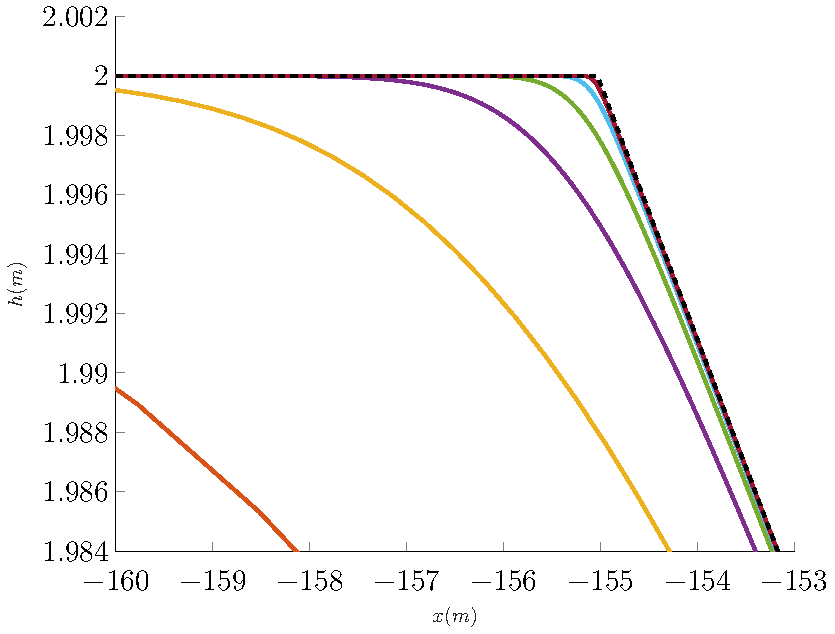
\includegraphics[width=\textwidth]{./Figures/Simulations/Validation/DBSWWE/hRFTop.pdf}
		\caption{Top of rarefaction fan}
	\end{subfigure}
	\caption{Plots of $h$ at $t=35s$ for the smooth dam-break problem around important locations with $\Delta x = 2^{-1}$ ({\color{mycolor1}\solidrule}), $2^{-2}$ ({\color{mycolor2}\solidrule}), $2^{-3}$ ({\color{mycolor3}\solidrule}), $2^{-4}$ ({\color{mycolor4}\solidrule}), $2^{-5}$ ({\color{mycolor5}\solidrule}), $2^{-6}$ ({\color{mycolor6}\solidrule}), $2^{-7}$ ({\color{mycolor7}\solidrule}), $2^{-8}$ ({\color{mycolor1}\solidrule}) and the analytic solution ({\dashedrule}) of the SWWE to the corresponding dam-break problem.}
	\label{Fig:Conv_Ex}
\end{figure}

%
Figure \ref{Fig:Conv_Ex} demonstrates that as $\Delta x$ decreases tje numerical solutions are converging to better resolve these critical locations. The behaviour of the bottom of the rarefaction fan is very similar to the top, and the behaviour of the solutions for $u$ and $G$ is similar, and so has been omitted. The convergence of the numerical methods is difficult to measure since the solutions are discontinuous, and so this more visual approach is used. In the presence of discontinuities the method is no longer expected to be fully second-order accurate, due to the use of the limiters, even so the method still possesses good convergence properties in the presence of the discontinuities.

Figure \ref{Fig:DB_Cons} shows the conservation properties of the numerical solutions as $\Delta x$ decreases. The conservation of $h$ and $G=uh$ is at round-off error and thus the error gets larger as $\Delta x$ decreases and the number of calculations increases. The conservation of $u$ is now only first-order, while the conservation of $\mathcal{E}$ doesn't improve as $\Delta x$ decreases. The drop in order for conservation of $u$ is due to the use of limiters which whilst making the numerical method total variation diminishing \cite{LeVeque-2002} and more robust, also result in the reconstruction becoming first-order near discontinuities. The lack of improvement in conservation of $\mathcal{E}$ is because the solutions are not sufficiently smooth, and thus do not satisfy all conservation equations \eqref{eq:gSGN} simultaneously \cite{Pu-2018-1361}. The loss of conservation in $\mathcal{H}$ is also a feature of the analytic solution as can be seen in Figure \ref{Fig:DB_Energy} which plots the total amount of energy over time for numerical and the analytic solutions. 
%
%Remove uh and energy, since energy dissipated anyway
\begin{figure}
	\centering
	\begin{subfigure}{0.49\textwidth}
		\centering
		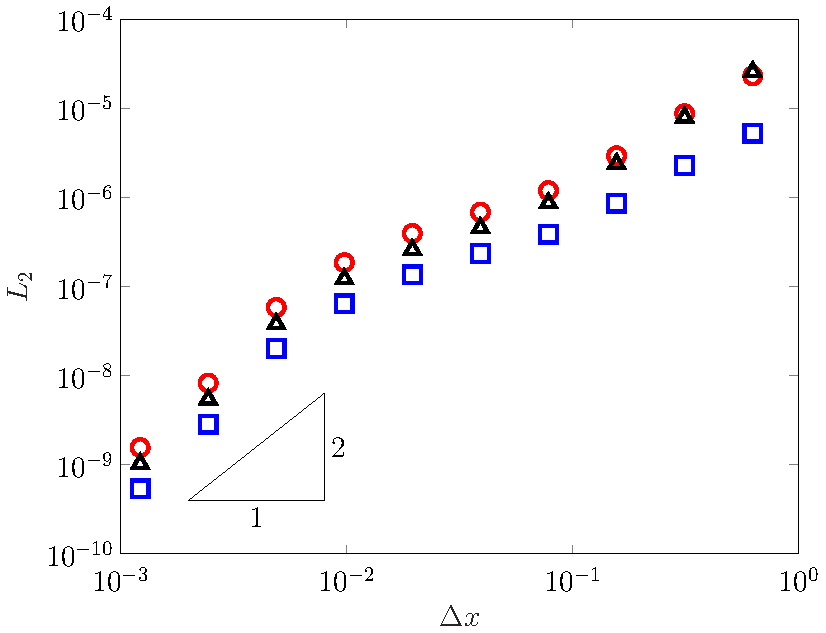
\includegraphics[width=\textwidth]{./Figures/Simulations/Validation/DBSWWE/ConvergenceInConstantState.pdf}
		\caption{$L_2$ for constant state with $u$ (\trianglet{black})}
		\label{Fig:DB_Comp_Conv}
	\end{subfigure}
	\begin{subfigure}{0.49\textwidth}
		\centering
	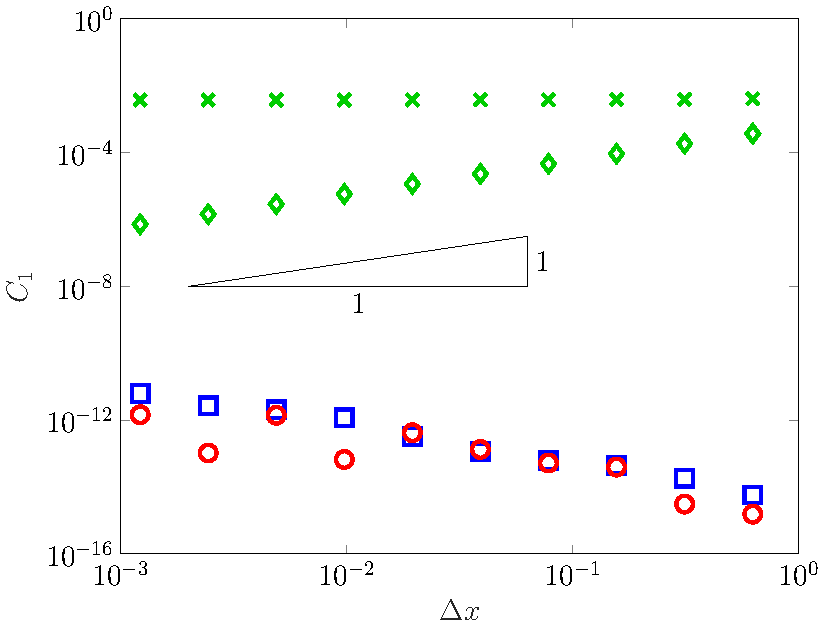
\includegraphics[width=\textwidth]{./Figures/Simulations/Validation/DBSWWE/EnergyResults.pdf}
\caption{$C_1$ with $uh$ (\trianglet{black})}
		\label{Fig:DB_Comp_Cons}
	\end{subfigure}
	\caption{Convergence and conservation plots for $h$ (\squaret{blue}) , $G$ (\circlet{red}), $\mathcal{E}$ (\crosst{green!80!black}) and $\mathcal{E}^*$ (\diamondt{green!80!black}) as $\Delta x$ varies.}
	\label{Fig:DB_Comp}
\end{figure}

\begin{figure}
	\centering
	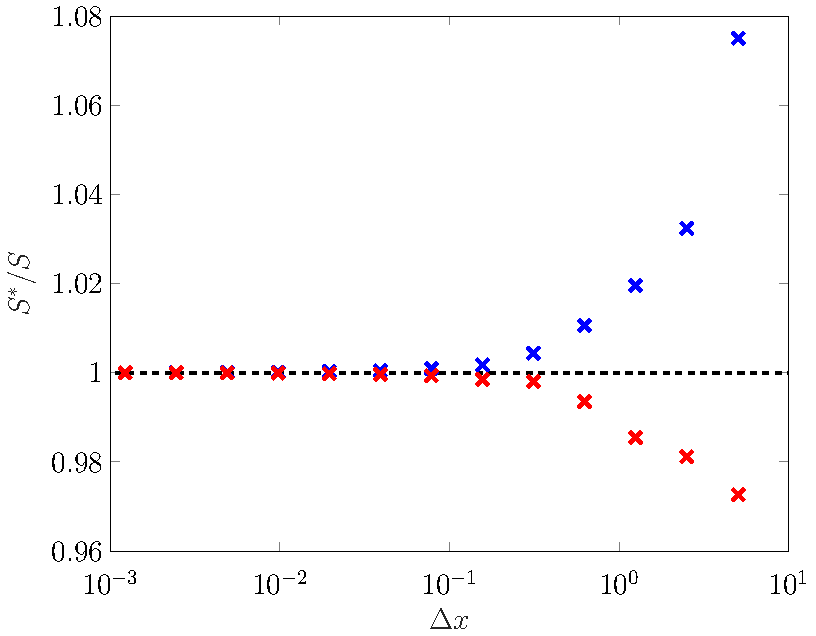
\includegraphics[width=0.5\textwidth]{./Figures/Simulations/Validation/DBSWWE/ShockSpeedEstimates.pdf}
	\caption{Estimates for Shock speed as $\Delta x \rightarrow 0$ lower bound (\crosst{red}) and upper bound (\crosst{blue}) .}
	\label{Fig:DB_ShockSpeed_Comp}
\end{figure}



These results demonstrate that the analytic solution of the SWWE has been accurately reproduced by the numerical method. 

\subsection{Forced Solutions}
To demonstrate the validity and versatility of the method to solve the gSGN for any $\beta$ values, forced solutions were used. To generate a forced solution the forced gSGN equations are considered
\begin{subequations}
	\begin{gather}
	\dfrac{\partial h}{\partial t} + \dfrac{\partial (uh)}{\partial x} = \dfrac{\partial h^*}{\partial t} + \dfrac{\partial (u^*h^*)}{\partial x} 
	\label{eq:gSGN_Gh_Forced}
	\end{gather}
	\begin{multline}
	\dfrac{\partial G }{\partial t}  + \dfrac{\partial}{\partial x} \left ( uG + \dfrac{gh^2}{2} - \beta_1 h^3\dfrac{\partial u}{\partial x}\dfrac{\partial u}{\partial x}  - \frac{1}{2} \beta_2 g h^2  \left[h\frac{\partial^2 h}{\partial x^2} + \frac{1}{2}\frac{\partial h}{\partial x}\frac{\partial h}{\partial x}\right]\right ) = \\ \dfrac{\partial G^* }{\partial t}  + \dfrac{\partial}{\partial x} \left ( u^*G^* + \dfrac{g\left(h^*\right)^2}{2} - \beta_1\left(h^*\right)^3\dfrac{\partial u^*}{\partial x}\dfrac{\partial u^*}{\partial x}  - \frac{1}{2} \beta_2 g \left(h^*\right)^2  \left[h^*\frac{\partial^2 h^*}{\partial x^2} + \frac{1}{2}\frac{\partial h^*}{\partial x}\frac{\partial h^*}{\partial x}\right]\right ).
	\label{eq:gSGN_GG_Forced}
	\end{multline}
	\label{eq:gSGN_Forced}
\end{subequations}
The forced gSGN admit the solutions $h^*$, $u^*$ and $G^*$ assuming $G^*$ appropriately satisfies \eqref{eq:G_divergent}. Since these equations are satisfied for any chosen $h^*$, $u^*$ and $G^*$ and any $\beta$ values, forced solutions can be used to verify the method for a large class of problems. Since the left hand-side of these modified equations are approximated by the numerical method, by combining the numerical method with the analytic expressions for the right hand-side, produces a method that approximates the forced gSGN equation with the same convergence properties as the underlying numerical method for the gSGN equations. 

Since $h^*$, $u^*$ and $G^*$ are arbitrary any desires solution can be generated and used to test the convergence properties for situations for which no known analytic solution to the equations exist. Of particular in this paper are solutions where the $\beta$ values are not equivalent to well studied equations and thus have no known analytic solutions exist, and where all the terms in the equations are non-zero, and thus must be approximated accurately. 

To accomplish these goals the following forced solutions
\begin{subequations}
	\begin{equation}
	h^*(x,t) = a_0 + a_1 \exp\left( \dfrac{\left(x - a_2 t\right)^2}{2 a_3} \right)
	\end{equation}
	\begin{equation}
	u^*(x,t) = a_4 \exp\left( \dfrac{\left(x - a_2 t\right)^2}{2 a_3} \right)
	\end{equation}
	\begin{align}
	\beta_1(x,t) &= a_6 \\
	\beta_2(x,t) &= a_7
	\end{align}
\end{subequations}
where $G^*$ is given by \eqref{eq:G_divergent}, were used. These forced solutions describe Gaussian bumps in $h$ and $u$ that travel at a constant speed $a_2$. The particular parameter values $a_0=1$, $a_1=0.5$, $a_3=20$, $a_4=0.3$, $a_6 = 1$ and $a_7=2$ were chosen in this investigation. Note that using these values, all terms in \eqref{eq:gSGN_G} are non-zero, and thus must be accurately approximated by the numerical method to reproduce the forced solution.

The numerical solutions were produced over the domain $\left[-100,100\right]$ with a final time of $t=10$. The spatial resolution was varied like so $\Delta x = 200 / (100 \times 2^{l})$, while the CFL condition was satisfied by setting $\Delta t = \Delta x  / \left( 2 \left[a_4 + a_2+ \sqrt{g \left(a_0 + a_1\right)}\right] \right)$. The acceleration due to gravity $g=9.81m^2/s$ and the limiting parameter $\theta = 1.2$ was used.

Figure \ref{Fig:FS_Ex} shows example numerical solutions at the final time for $h$, $G$ and $u$ with $\Delta x = 200 / (100 \times 2^{6}) \approx 0.03$. These example solutions demonstrate that the numerical method is able to reproduce the forced solution well.
%
\begin{figure}
	\centering
	\begin{subfigure}{0.32\textwidth}
		\centering
		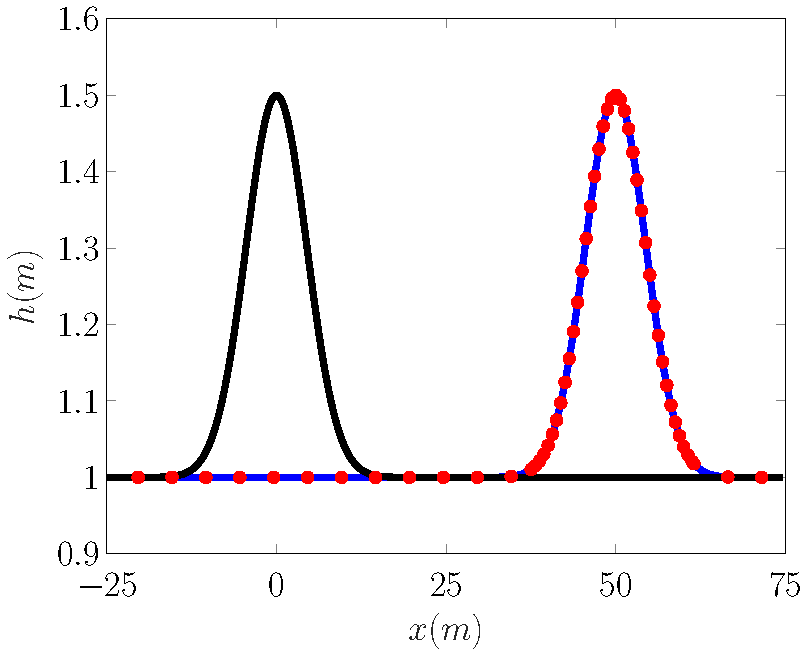
\includegraphics[width=\textwidth]{./Figures/Simulations/Validation/Forced/iSGN/h.pdf}
		\caption{$h$}
	\end{subfigure}
	\begin{subfigure}{0.32\textwidth}
		\centering
		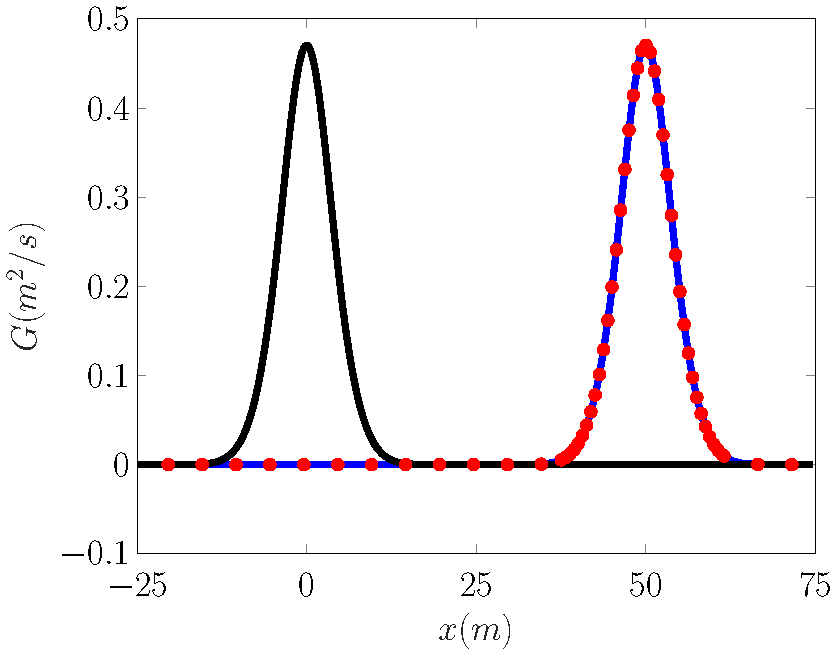
\includegraphics[width=\textwidth]{./Figures/Simulations/Validation/Forced/iSGN//G.pdf}
		\caption{$G$}
	\end{subfigure}
	\begin{subfigure}{0.32\textwidth}
		\centering
		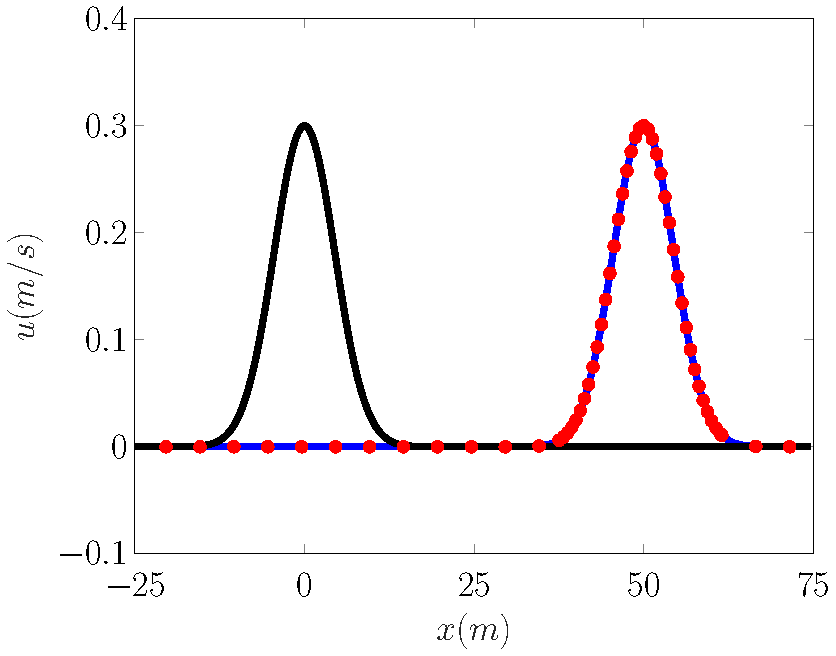
\includegraphics[width=\textwidth]{./Figures/Simulations/Validation/Forced/iSGN/u.pdf}
		\caption{$u$}
	\end{subfigure}
	\caption{Example plots Initial (\solidrule), analytic solution ({\color{blue}\solidrule}), and numerical solution with $\Delta x \approx 0.03m$ (\tikzcircle{red}).}
	\label{Fig:FS_Ex}
\end{figure}

Figure \ref{Fig:FS_Conv} demonstrates the convergence of the numerical scheme as $\Delta x$ decreases. All quantities of interest are converging at the expected second-order. Since the RHS is given analytically, the observed error is caused by the numerical method. Therefore, these results demonstrate that the scheme is second-order for all terms in gSGN equations. Unfortunately, to be able to accurately reproduce the forced solutions the limiting on the derivatives had to be removed. This made the derivative approximations consistent, and importantly didn't restrict the derivatives at the top of the Gaussian bumps. Thus the forced solutions only validate the method without derivative limiting for all $\beta$ values. However, given that the limiting is only comparing derivative approximations of the same order and the above analytic solutions, the numerical method is well validated.
%
\begin{figure}
	\centering
	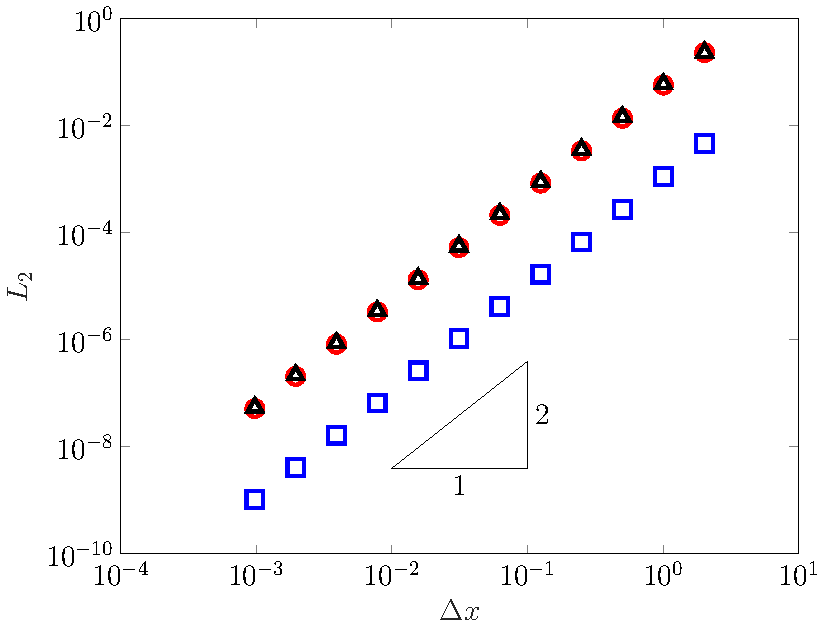
\includegraphics[width=0.49\textwidth]{./Figures/Simulations/Validation/Forced/iSGN/NormResults.pdf}
	\caption{Convergence plot of $h$ (\squaret{blue}) , $G$ (\circlet{red}), $u$ (\trianglet{black}) for the forced solutions for various $\Delta x$ values.}
	\label{Fig:FS_Conv}
\end{figure}


\section{Conclusion}
A modified version of the SGN solver outlined by \citet{Zoppou-etal-2017} was used to solved the gSGN equations which make the constant in front of the dispersive term free and adds a surface tension-like regularisation term \cite{Clamond-et.al-2017-245,Clamond-Dutykh-2018-237}. The new gSGN solver was validated against analytic solutions of the SGN and SWWE equations and forced solutions. The analytic solutions demonstrate that the gSGN solver accurately reproduces important members of the gSGN family of equations whilst conserving the quantities of interest for sufficiently smooth solutions, and the forced solutions demonstrate that the method remains second-order for all values of the free parameters, $\beta_1$ and $\beta_2$. The gSGN method described above is the first well validated numerical method for the gSGN equations and the rSWWE and iSGN families of equations. The numerical method is then used to verify and expand numerical results in the literature for the smoothed dam-break problem \cite{Clamond-Dutykh-2018-237,Clamond-et.al-2017-245,Pu-2018-1361}. The first set of these experiments demonstrate the rSWWE family possesses regularised numerical solutions that converge nicely as the SWWE are approached. Additionally, the numerical results for energy dissipation agree with the analytic result of \citet{Pu-2018-1361}, where the weak singularities associated with this dissipation can be seen in plots of the conserved quantity $G$. The second group of experiments demonstrate the behaviour of the iSGN family of equations, which agrees very well with the linear theory. The results demonstrate that for steep gradient problems the iSGN family will require higher resolution grids or higher order methods to resolve the dispersive wave train around the high wave-number limits. Finally, the numerical solutions for the family of equations that lie between the SGN and SWWE equations, the SGN to SWWE family were studied. These results demonstrate that even for very small $\beta_1$ values steep gradients will develop extensive dispersive wave trains and when $\beta_1$ is close to the critical SWWE value, then the solutions of the SGN to SWWE family dissipate energy at the same rate as the SWWE for the numerical solutions. 

\bibliographystyle{unsrtnat}
\bibliography{Bibliography}


\end{document} 